%%
%% Copyright 2007, 2008, 2009 Elsevier Ltd
%%
%% This file is part of the 'Elsarticle Bundle'.
%% ---------------------------------------------
%%
%% It may be distributed under the conditions of the LaTeX Project Public
%% License, either version 1.2 of this license or (at your option) any
%% later version.  The latest version of this license is in
%%    http://www.latex-project.org/lppl.txt
%% and version 1.2 or later is part of all distributions of LaTeX
%% version 1999/12/01 or later.
%%
%% The list of all files belonging to the 'Elsarticle Bundle' is
%% given in the file `manifest.txt'.
%%

%% Template article for Elsevier's document class `elsarticle'
%% with numbered style bibliographic references
%% SP 2008/03/01
%%
%%
%%
%% $Id: elsarticle-template-num.tex 4 2009-10-24 08:22:58Z rishi $
%%
%%
\documentclass[final,5p]{elsarticle}

%% Use the option review to obtain double line spacing
%% \documentclass[preprint,review,12pt]{elsarticle}

%% Use the options 1p,twocolumn; 3p; 3p,twocolumn; 5p; or 5p,twocolumn
%% for a journal layout:
%% \documentclass[final,1p,times]{elsarticle}
%% \documentclass[final,1p,times,twocolumn]{elsarticle}
%% \documentclass[final,3p,times]{elsarticle}
%% \documentclass[final,3p,times,twocolumn]{elsarticle}
%% \documentclass[final,5p,times]{elsarticle}
%% \documentclass[final,5p,times,twocolumn]{elsarticle}

%% if you use PostScript figures in your article
%% use the graphics package for simple commands
%% \usepackage{graphics}
%% or use the graphicx package for more complicated commands
%% \usepackage{graphicx}
%% or use the epsfig package if you prefer to use the old commands
%% \usepackage{epsfig}

%% The amssymb package provides various useful mathematical symbols
\usepackage{amssymb}
%% The amsthm package provides extended theorem environments
%% \usepackage{amsthm}

%% The lineno packages adds line numbers. Start line numbering with
%% \begin{linenumbers}, end it with \end{linenumbers}. Or switch it on
%% for the whole article with \linenumbers after \end{frontmatter}.
%% \usepackage{lineno}

%% natbib.sty is loaded by default. However, natbib options can be
%% provided with \biboptions{...} command. Following options are
%% valid:

%%   round  -  round parentheses are used (default)
%%   square -  square brackets are used   [option]
%%   curly  -  curly braces are used      {option}
%%   angle  -  angle brackets are used    <option>
%%   semicolon  -  multiple citations separated by semi-colon
%%   colon  - same as semicolon, an earlier confusion
%%   comma  -  separated by comma
%%   numbers-  selects numerical citations
%%   super  -  numerical citations as superscripts
%%   sort   -  sorts multiple citations according to order in ref. list
%%   sort&compress   -  like sort, but also compresses numerical citations
%%   compress - compresses without sorting
%%
%% \biboptions{comma,round}

%\biboptions{comma,round}

\usepackage{graphicx}
\usepackage[space]{grffile}
\usepackage{latexsym}
\usepackage{amsfonts,amsmath,amssymb}
\usepackage{url}
\usepackage[utf8]{inputenc}
\usepackage{fancyref}
\usepackage{hyperref}
\usepackage{caption}
\hypersetup{colorlinks=false,pdfborder={0 0 0},}

\newcommand{\truncateit}[1]{\truncate{0.8\textwidth}{#1}}
\newcommand{\scititle}[1]{\title[\truncateit{#1}]{#1}}
\usepackage{comment}
\newcommand{\unit}[1]{\ensuremath{\, \mathrm{#1}}}

\usepackage[usenames,dvipsnames,svgnames,table]{xcolor}

\newcommand{\aj}{AJ}			% Astronomical Journal
\newcommand{\araa}{ARA\&A}		% Annual Review of Astron and Astrophys
\newcommand{\apj}{ApJ}			% Astrophysical Journal
\newcommand{\apjl}{ApJLett}		% Astrophysical Journal, Letters
\newcommand{\apjlett}{ApJLett}		% Astrophysical Journal, Letters
\newcommand{\apjs}{ApJS}		% Astrophysical Journal, Supplement
\newcommand{\apjsupp}{ApJS}		% Astrophysical Journal, Supplement
\newcommand{\ao}{Appl.~Opt.}		% Applied Optics
\newcommand{\apss}{Ap\&SS}		% Astrophysics and Space Science
\newcommand{\aap}{A\&A}			% Astronomy and Astrophysics
\newcommand{\astap}{A\&A}		% Astronomy and Astrophysics
\newcommand{\aapr}{A\&A~Rev.}		% Astronomy and Astrophysics Reviews
\newcommand{\aaps}{A\&AS}		% Astronomy and Astrophysics, Supplement
\newcommand{\azh}{AZh}			% Astronomicheskii Zhurnal
\newcommand{\baas}{BAAS}		% Bulletin of the AAS
\newcommand{\jrasc}{JRASC}		% Journal of the RAS of Canada
\newcommand{\memras}{MmRAS}		% Memoirs of the RAS
\newcommand{\mnras}{MNRAS}		% Monthly Notices of the RAS
\newcommand{\pra}{Phys.~Rev.~A}		% Physical Review A: General Physics
\newcommand{\prb}{Phys.~Rev.~B}		% Physical Review B: Solid State
\newcommand{\prc}{Phys.~Rev.~C}		% Physical Review C
\newcommand{\prd}{Phys.~Rev.~D}		% Physical Review D
\newcommand{\pre}{Phys.~Rev.~E}		% Physical Review E
\newcommand{\prl}{Phys.~Rev.~Lett.}	% Physical Review Letters
\newcommand{\pasp}{PASP}		% Publications of the ASP
\newcommand{\pasj}{PASJ}		% Publications of the ASJ
\newcommand{\qjras}{QJRAS}		% Quarterly Journal of the RAS
\newcommand{\revmodphys}{Rev.\ Mod.\ Phys.} %Rev Mod Phys
\newcommand{\skytel}{S\&T}		% Sky and Telescope
\newcommand{\solphys}{Sol.~Phys.}	% Solar Physics
\newcommand{\sovast}{Soviet~Ast.}	% Soviet Astronomy
\newcommand{\ssr}{Space~Sci.~Rev.}	% Space Science Reviews
\newcommand{\zap}{ZAp}			% Zeitschrift fuer Astrophysik
\newcommand{\nat}{Nature}		% Nature
\newcommand{\iaucirc}{IAU~Circ.}       	% IAU Circulars
\newcommand{\aplett}{Astrophys.~Lett.} 	% Astrophysics Letters
\newcommand{\apspr}{Astrophys.~Space~Phys.~Res.}% Astrophysics Space Physics Research
\newcommand{\fcp}{Fund.~Cosmic~Phys.}  % Fundamental Cosmic Physics
\newcommand{\gca}{Geochim.~Cosmochim.~Acta}   % Geochimica Cosmochimica Acta
\newcommand{\grl}{Geophys.~Res.~Lett.} % Geophysics Research Letters
\newcommand{\jcp}{J.~Chem.~Phys.}	% Journal of Chemical Physics
\newcommand{\jgr}{J.~Geophys.~Res.}	% Journal of Geophysics Research
\newcommand{\nphysa}{Nucl.~Phys.~A}   % Nuclear Physics A
\newcommand{\physrep}{Phys.~Rep.}   % Physics Reports
\newcommand{\physscr}{Phys.~Scr}   % Physica Scripta
\newcommand{\planss}{Planet.~Space~Sci.}   % Planetary Space Science
\newcommand{\procspie}{Proc.~SPIE}   % Proceedings of the SPIE

\usepackage{relsize}
\newcommand\Cpp{C\nolinebreak[4]\hspace{-.05em}\raisebox{.4ex}{\relsize{-3}{\textbf{++}}}}


\definecolor{midgray}{gray}{0.85}%

\usepackage{listings}


\lstdefinestyle{code}{%
     basicstyle=\footnotesize\ttfamily,       
     frame=single,               
     framesep=1pt,               
     framerule=0.8pt,            
     rulecolor=\color{midgray},  
     breaklines=true,           
     breakindent=0pt,
     backgroundcolor=\color{midgray},
     prebreak=\mbox{\textbackslash{}}             
}

\lstdefinestyle{python}{
  style=code,
  belowcaptionskip=1\baselineskip,
  breaklines=true,
  frame=single,
  framesep=2pt,
  xleftmargin=\parindent,
  language=Python,
  showstringspaces=false,
  basicstyle=\footnotesize\ttfamily,
  keywordstyle=\bfseries\color{green!40!black},
  commentstyle=\itshape\color{gray},
  identifierstyle=\color{black},
  stringstyle=\color{gray},
  rulecolor=\color{midgray}, 
}

\lstdefinestyle{java}{
  style=python,
  language=Java
}





\journal{Astronomy and Computing}

\begin{document}

\begin{frontmatter}

%% Title, authors and addresses

%% use the tnoteref command within \title for footnotes;
%% use the tnotetext command for the associated footnote;
%% use the fnref command within \author or \address for footnotes;
%% use the fntext command for the associated footnote;
%% use the corref command within \author for corresponding author footnotes;
%% use the cortext command for the associated footnote;
%% use the ead command for the email address,
%% and the form \ead[url] for the home page:
%%
%% \title{Title\tnoteref{label1}}
%% \tnotetext[label1]{}
%% \author{Name\corref{cor1}\fnref{label2}}
%% \ead{email address}
%% \ead[url]{home page}
%% \fntext[label2]{}
%% \cortext[cor1]{}
%% \address{Address\fnref{label3}}
%% \fntext[label3]{}

\title{Iris: an Extensible Application for Building and Analyzing\\
Spectral Energy Distributions}

\author[sao]{Omar Laurino~\corref{cor}}
\cortext[cor]{Corresponding author}
\ead{olaurino@cfa.harvard.edu}

\author[sao]{Jamie Budynkiewicz}
%\ead{jbudynkiewicz@cfa.harvard.edu}

\author[sao]{Raffaele D'Abrusco}
%\ead{dabrusco@head.cfa.harvard.edu}

\author[sao]{Nina Bonaventura~\fnref{nina}}
\fntext[nina]{Present Affiliation: McGill University, 3600 University St.
Montr\'{e}al QC, Canada H3A 2T8}
%\ead{nina.bonaventura@mail.mcgill.ca}

\author[stsci]{Ivo Busko}
%\ead{busko@stsci.edu}

\author[sao]{Mark Cresitello-Dittmar}
%\ead{mdittmar@cfa.harvard.edu}

\author[sao]{Stephen M. Doe}
%\fntext[doe]{ADD}
%\ead{stephen.m.doe@gmail.com}

\author[ipac]{Rick Ebert}
%\ead{rick@ipac.caltech.edu}

\author[sao]{Janet D. Evans}
%\ead{jdeponte@cfa.harvard.edu}

\author[noao]{Patrick Norris}
%\ead{norris@noao.edu}

\author[ipac]{Olga Pevunova}
%\ead{olga@ipac.caltech.edu}

\author[sao]{Brian Refsdal}
%\fntext[brian]{ADD}
%\ead{brian.refsdal@gmail.com CHANGE}

\author[noao]{Brian Thomas}

\author[stsci]{Randy Thompson}
%\ead{rthompson@stsci.edu}

%% Addresses
\address[sao]{Smithsonian Astrophysical Observatory, 60 Garden St.
Cambridge, MA 02138}
\address[stsci]{Space Telescope Science Institute, 3700 San Martin Dr.
Baltimore, MD 21218}
\address[ipac]{Infrared Processing and Analysis Center, 770 South Wilson Ave.
Pasadena, CA 91125}
\address[noao]{National Optical Astronomy Observatory, 950 N Cherry Ave.
Tucson, AZ 85719}

\begin{abstract}
Iris is an extensible application that provides astronomers with a user-friendly user interface capable of ingesting broad-band data from many different sources in order to build, explore, and model spectral energy distributions (SEDs). Iris takes advantage of the standards defined by the International Virtual Observatory Alliance, but hides the technicalities of such standards by implementing different layers of abstraction on top of them. Such intermediate layers provide hooks that users and developers can exploit in order to extend the functionalities provided by Iris. For instance, custom Python models can be combined in arbitrary ways with the Iris built-in models or with other custom functions. As such, Iris offers a platform for the development and integration of SED data, services, and applications, either from the user's system or from the web. In this paper we describe the built-in features provided by Iris for building and analyzing SEDs. We also explore in some detail the Iris framework and software development kit, showing how astronomers and software developers can plug their code into an integrated SED analysis environment.
\end{abstract}




%\begin{keyword}
%% keywords here, in the form: keyword \sep keyword

%% MSC codes here, in the form: \MSC code \sep code
%% or \MSC[2008] code \sep code (2000 is the default)

%\end{keyword}

\end{frontmatter}

\bibliographystyle{model2-names}


\label{sec:introduction}
\section{Introduction}
The International Virtual Observatory Alliance~\citep[IVOA;][]{2004SPIE.5493..137Q} provides a set of standards and protocols that enable interoperability among astronomy-centered services and applications. In order to design effective applications, one wants to leverage IVOA standards and protocols without exposing the complexity and technicality of their specifications to the users. Also, while application developers implement many desired functionalities, they must keep the door open for plugging in user's analysis code, and allow third party developers to extend the application's functionality without being aware of the standards themselves. Designing such general purpose applications thus becomes an exercise in designing a framework that implements some basic, effective functionality for a wide set of use cases, while being highly extensible.

%Iris, the Virtual Astronomical Observatory~\citep[VAO;][]{2012SPIE.8449E..0HB} spectral energy distribution (SED) analysis tool, is such an IVOA-enabled application. Iris was developed to provide the astronomical community a desktop application for building, viewing and modeling broadband spectro-photometric SEDs, while implementing IVOA standards and protocols and taking advantage of existing astronomy software~\citep{2012ASPC..461..893D,2013AAS...22124038L}. 

Iris, the Virtual Astronomical Observatory~\citep[VAO;][]{2012SPIE.8449E..0HB} spectral energy distribution (SED) analysis tool, is such an IVOA-enabled desktop application for building, viewing and modeling broadband spectro-photometric SEDs. While implementing IVOA standards and protocols, the Iris development team took advantage of existing astronomy software~\citep{2012ASPC..461..893D,2013AAS...22124038L}, namely Specview\footnote{ascl.net/1210.016} for the visualization and fitting user interfaces, the NASA/IPAC Extragalactic Database (NED) SED Service for data acquisition, and Sherpa\footnote{ascl.net/1107.005} for the modeling and fitting engine. Along with these components, new ones, like the SED Builder, were deveoped specifically for Iris. 

%The team took advantage of several existing astronomy software packages, namely Specview for the visualization and fitting user interfaces, the NASA/IPAC Extragalactic Database (NED) SED Service for data acquisition, and Sherpa for the modeling and fitting engine. The VAO also developed SED Builder for Iris, which handles SED data I/O and management with IVOA standards. 

With Iris users may populate SEDs with data from files, built-in portals to data archives, and other Virtual Observatory (VO) applications; they can interactively visualize and edit SEDs, and fit SEDs with fine-tuned modeling features. Users may choose from a suite of provided astrophysical models, or load their own Python functions and template libraries. All front-end features of Iris completely hide the underlying technical VO standards and protocols from the user.

%Iris is composed of several existing astronomy packages loosely coupled together to provide the main capabilities, namely Specview for the visualization and fitting user interfaces, the NASA/IPAC Extragalactic Database (NED) SED Service for data acquisition, and Sherpa for the modeling and fitting engine. The VAO also developed SED Builder, which handles SED data I/O and management in Iris. Together with other interoperable features, 

%With Iris, users may populate SEDs with data from files, built-in portals to data archives, and other Virtual Observatory (VO) applications. 
%%Iris is lenient on the data format, so while it natively supports VO-compliant files (properly annotated VOTABLE and FITS files), Iris can ingest ASCII, CSV, and other table-like formats with some user input. 
%The application also provides interactive data visualization and editing tools, and a SED fitting tool for fine-tuned modeling. Users may choose from a suite of provided astrophysical models, or load their own Python functions and template libraries. All front-end features of Iris completely hide the underlying technical VO standards and protocols from the user.

%%Iris was devoted to provide functionality in a specific scientific domain, namely the analysis of broad-band SEDs. This requirement clearly defines the semantic scope of the  Iris extensible framework, and provides a clear abstraction layer to both users and developers, inside and outside of the development team.

Iris was developed inside the framework of the VAO science applications: the different components were contributed by developers from the Smithsonian Astrophysical Observatory, the Space Telescope Science Institute, and the NASA Infrared Processing and Analysis Center. Quality Assurance and testing were lead by team members at the National Optical Astronomy Observatory and Space Telescope Science Institute.

In this paper we present the Iris application, its design, and how its architecture makes Iris extensible through the use of plug-ins. In section \ref{sec:overview} we briefly explore the landscape of SED applications and analysis tools which Iris joined, and provide an example use-case of Iris. We explore how astronomers can include their own models or templates as Python functions in section \ref{sec:usermodels}. An introduction to the Iris' general architecture (the Iris \emph{stack}) is illustrated in section \ref{sec:stack}. A more detailed overview of the Iris extensible framework design (section \ref{sec:architecture}) is followed by a detailed description of the more advanced Iris functionalities (section \ref{sec:components}). Finally, we describe the Iris software development kit, including a ``How-to'' on extending Iris with plug-ins (section \ref{sec:plugins}).

Sections \ref{sec:architecture} and \ref{sec:plugins} are targeted to software developers.

The paper refers to version 2.0.1 of Iris. Iris can be downloaded as a binary archive for Mac OS X and Linux\footnote{\url{http://cxc.cfa.harvard.edu/iris/latest/download/}}, and the source code is hosted on GitHub as a public repository\footnote{\url{https://github.com/ChandraCXC/iris}}.

\section{SED Analysis with Iris}
\label{sec:overview}

Fitting spectral energy distributions allows astronomers to estimate fundamental physical properties like stellar mass, star formation rates, dust content and overall environments of astronomical objects (e.g. \citep{1998AJ....115.1329S}, \citep{2001ApJS..137..139S}, \citep{2007ApJS..169..328R}, and many others). With deeper wide-field surveys and increasing numbers of datasets over the years, astronomers have been able to use multi-wavelength SEDs more frequently for their research. As such, many robust SED analysis codes have been created to help astronomers model, fit, and derive physical quantities from SEDs \citep{2011Ap&SS.331....1W,2013ARA&A..51..393C}. These widely-used codes implement a diverse set of methods, for instance: inversion (\texttt{PAHFIT} \citep{2007ApJ...656..770S}, \texttt{STAR\-LIGHT} \cite{2004MNRAS.355..273C}), principal component analysis \citep{2009MNRAS.394.1496B}, $\mathrm{\chi}^{2}$-minimization codes (\texttt{Le Phare} \citep{1999MNRAS.310..540A}, \texttt{hyperz} \citep{2000A&A...363..476B}), and Bayesian inference (\texttt{GalMC} \citep{2011ApJ...737...47A}; \texttt{VOSA} \citep{2008A&A...492..277B}; \texttt{BPZ} \citep{2000ApJ...536..571B}).

Most distributed fitting packages are tailored for specific data sets or spectral ranges (e.g. \texttt{PAHFIT}, \texttt{STAR\-LIGHT}), providing robust fitting methods and results. They require the data to be in a specific format with specific units in order for the tool to work properly. When fitting a broadband SED that spans over decades in the spectrum, the astronomer will typically gather datasets from different public archives and colleagues in order to add such data to their own. More often than not, the datasets are stored in different file formats and units. 
%and converting the data to an ingestible format becomes a tedious task.
The user must provide their own methods to extract the necessary data from each file, homogenize the units, and output a file in the format supported by the tool; converting the data to a supported format may easily become a tedious task with each additional dataset.

While SED analysis tools often have different input formats from each other, they effectively require the same information to run. Whether datasets are stored in a FITS file, a tab separated ASCII table, or a VOTable coming from a VO Data Discovery application, they are all serializations of the same, global, abstract, scientific model of spetral and photometric measurements for astronomical sources.

By employing a standardized definition of such model, Iris can can streamline the process of building SEDs for analysis: in other terms, one of the goals of Iris it to make SED building a painless and straightforward process, letting the scientist focus on the sophisticated and original parts of the scientific workflow: data analysis, hypothesis testing, and knowledge extraction.

Following VO efforts to seamlessly combine data services and applications, Iris offers an interface for building large broadband SEDs from different sources in various data formats, while providing robust fitting methods and interactive visualization capabilities using existing astronomical software.

It is important to stress that this is not only a matter of ingesting non-standard files, but also to allow scientists to create standardized versions of their datasets: the improved interoperability enables more tools, inside or outside Iris, to load and interpret such datasets with minimal user intervention.

Much effort has been put in making Iris lenient on the data format: natively supporting VO-compliant files (properly annotated VOTABLE~\citep{2011arXiv1110.0524O} and FITS files), Iris can ingest ASCII, CSV, and other table-like formats with some extra user input. Users may also seamlessly transfer data from other VO applications or data archive services through SAMP, the Simple Application Messaging Protocol~\citep{2011arXiv1110.0528T}.

But more importantly, Iris provides standardized views of the integrated datasets to its clients, whether they are built-in components, third party plugin-ins, or external applications.

%Iris is meant to be an open box SED analysis tool. If Iris is missing certain functionality, the user may develop a plugin for that functionality and add it to Iris. Thus, a user can employ Iris' SED building capabilites while running custom analysis, which in theory could be one of the fitting packages discussed above. %We explore this possibility in detail in Section \ref{sec:plugins}

To showcase its main functionalities, we present a brief, illustrative use-case of Iris usage: in the next sections we outline the analysis of the broadband SED of the flat spectrum radio quasar (FRSQ) object PKS 1127-14, and save the results to file. This is only a brief overview of a possible user thread, and more information about the individual Iris components introduced in this section are then described in more detail in the remainder of the paper.

% However, most SED analysis tools require similar data and pre-processing steps, like gathering and converting the data to compliant formats for the tools. Thus it becomes only a matter of providing an interoperable framework that makes building, viewing, and analyzing SEDs a straightforward process.

%Users can input SED data from a local file or a URL, with high leniency on the data format. Users may also beam data from other VO-enabled applications or data archive services through SAMP, the VAO-developed Simple Application Messaging Protocol~\citep{2011arXiv1110.0528T}. If the data format follows the IVOA Spectrum Data Model v1.03 \citep{2012arXiv1204.3055M}, or in other words a VO-compliant VOTable or FITS file, the data is read-in without any input by the user; otherwise, the user supplies the units and mapping to the spectral-flux coordinates in the file.

%While each code is tailored for specific datasets or object types, most SED analysis tools share similar necessities and require the same pre-processing steps. Thus it is worth developing an interoperable SED tool that Following VO efforts to seamlessly combine data services and applications, Iris offers a standard means of building large broadband SEDs from different sources in various data formats, while providing robust fitting methods and interactive visualization capabilities.

%[FIX ME: make me a happy, positive statement] While these exacting steps are worthwhile for the quality fitting results, gathering, pre-processing, and converting data to plug it in to a fitting engine should be standard/interpoerable and straightfoward.

%This inconvenience -- building SEDs from multiple sources -- drove a part of Iris' SED analysis design. Following VO efforts to seamlessly combine data services and applications, Iris offers a standard means of building large broadband SEDs from different sources in various data formats, while providing robust fitting methods and interactive visualization capabilities. Users can input SED data from a local file or a URL, with high leniency on the data format. Users may also beam data from other VO-enabled applications or data archive services through SAMP (Simple Application Messaging Protocol; \citep{2011arXiv1110.0528T}). If the data format follows the IVOA Spectrum Data Model v1.03 \citep{2012arXiv1204.3055M}, or in other words a VO-compliant VOTable or FITS file, the data is read-in without any input by the user; otherwise, the user supplies the units and  mapping to the spectral-flux coordinates in the file. How this method works is described in Section \ref{sec:components}.

%Users can input SED data from a local file, a URL, another VO-enabled application, or directly from VO-enabled data archive services, with high leniency on the data format.

%\begin{comment}
%Following the VO effort for seamless interoperability between data services and applications,

%The Virtual Observatory is an effort to standardize data formats and services so that users can seamlessly exchange data back and forth between archives and applications.
%
%Iris offers a standard means of building large broadband SEDs from different sources in various data formats, while providing robust fitting methods and interactive visualization capabilities.
%\end{comment}


\subsection{A Use Case}
\label{subsec:usecase}

\begin{figure*}
\centering
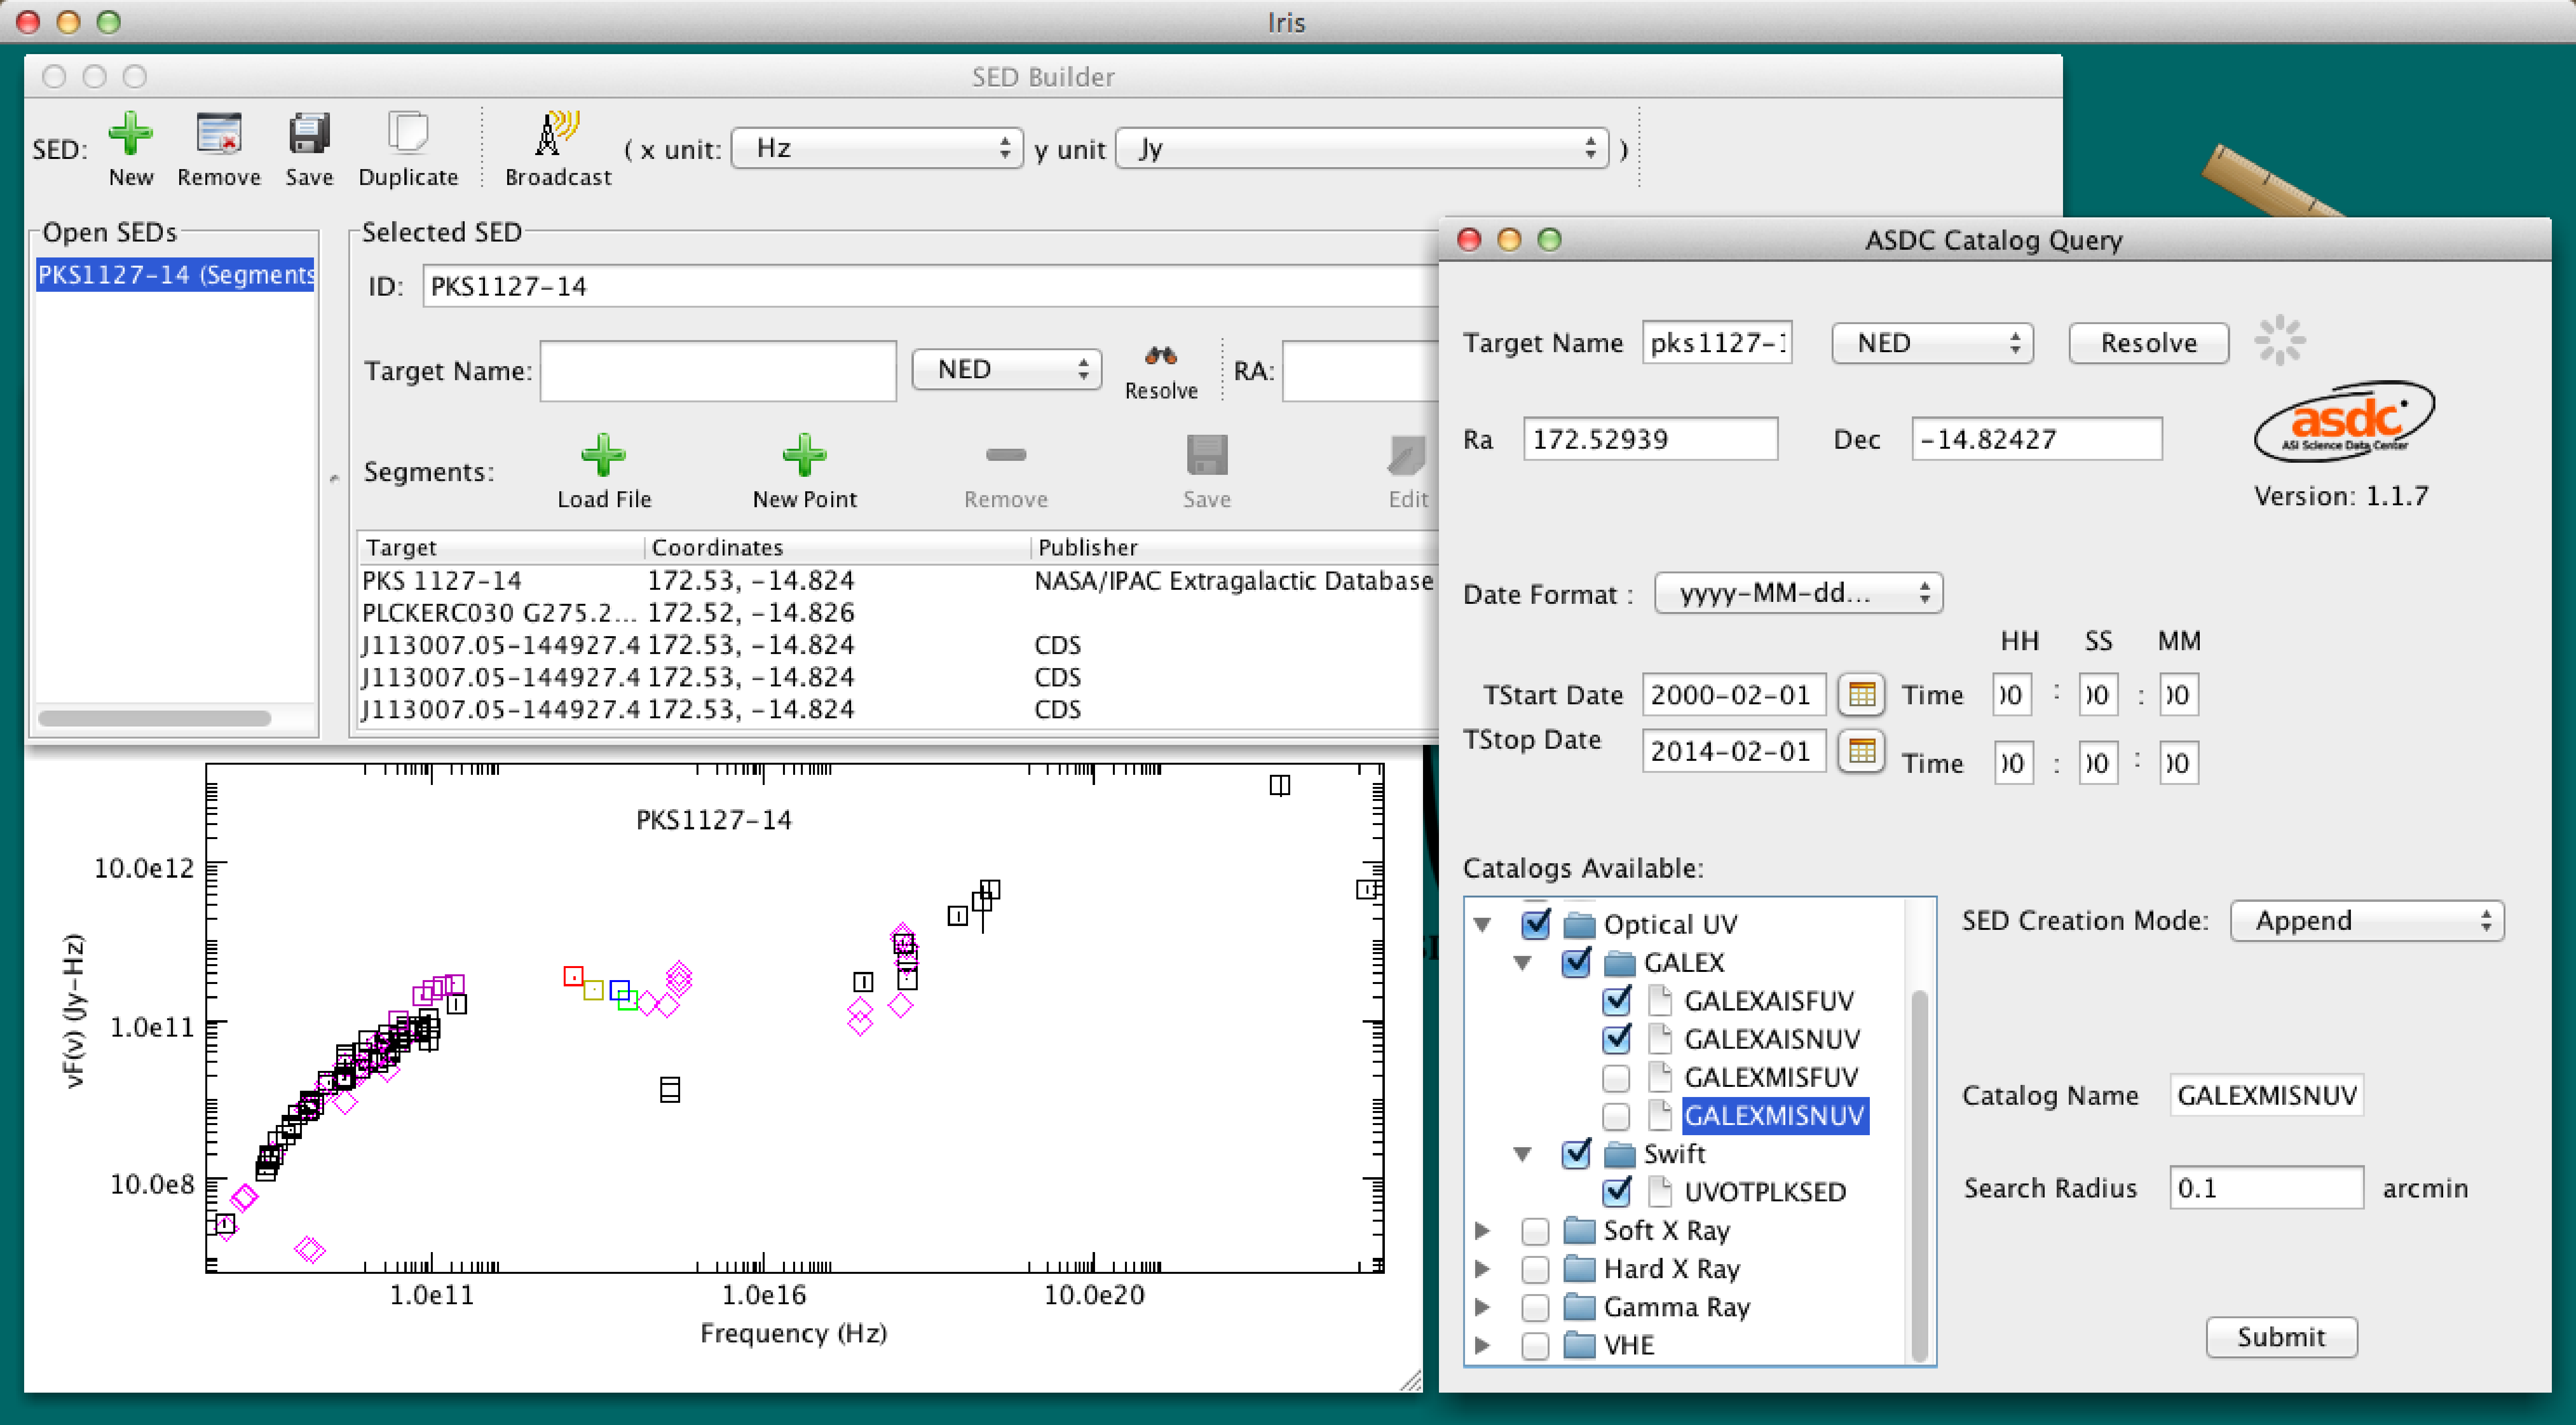
\includegraphics[height=0.3\textheight]{figures/built-in-visuals-loading1.png}
\caption{\textbf{Building the SED of blazar PKS 1127-14 in Iris} \textit{Top-left:} Data from the NED SED Service, a local file, and from TOPCAT are managed in the SED Builder. \textit{Bottom-left:} The various data Segments plotted in $\mathrm{\nu F \left( \nu \right)}$ units inside the SED Viewer. Squares show data with flux uncertainties, whereas the pink diamonds denote points without associated uncertainties. Each Segment in the SED Builder is plotted in a different color. Black squares are the data taken from NED; the pink sqaures in the radio are the data from PLANCK; and the red, yellow, blue, and green squares in the near-IR are the for WISE bands. \textit{Right:} An ASDC Data Query form for PKS 1127-14. The user searches for data between specified dates and available instruments (Swift and GALEX in this case). The data has been added to the open SED \texttt{PKS1127-14}.}
\label{fig:load_data}
\end{figure*}

\begin{figure*}
\centering
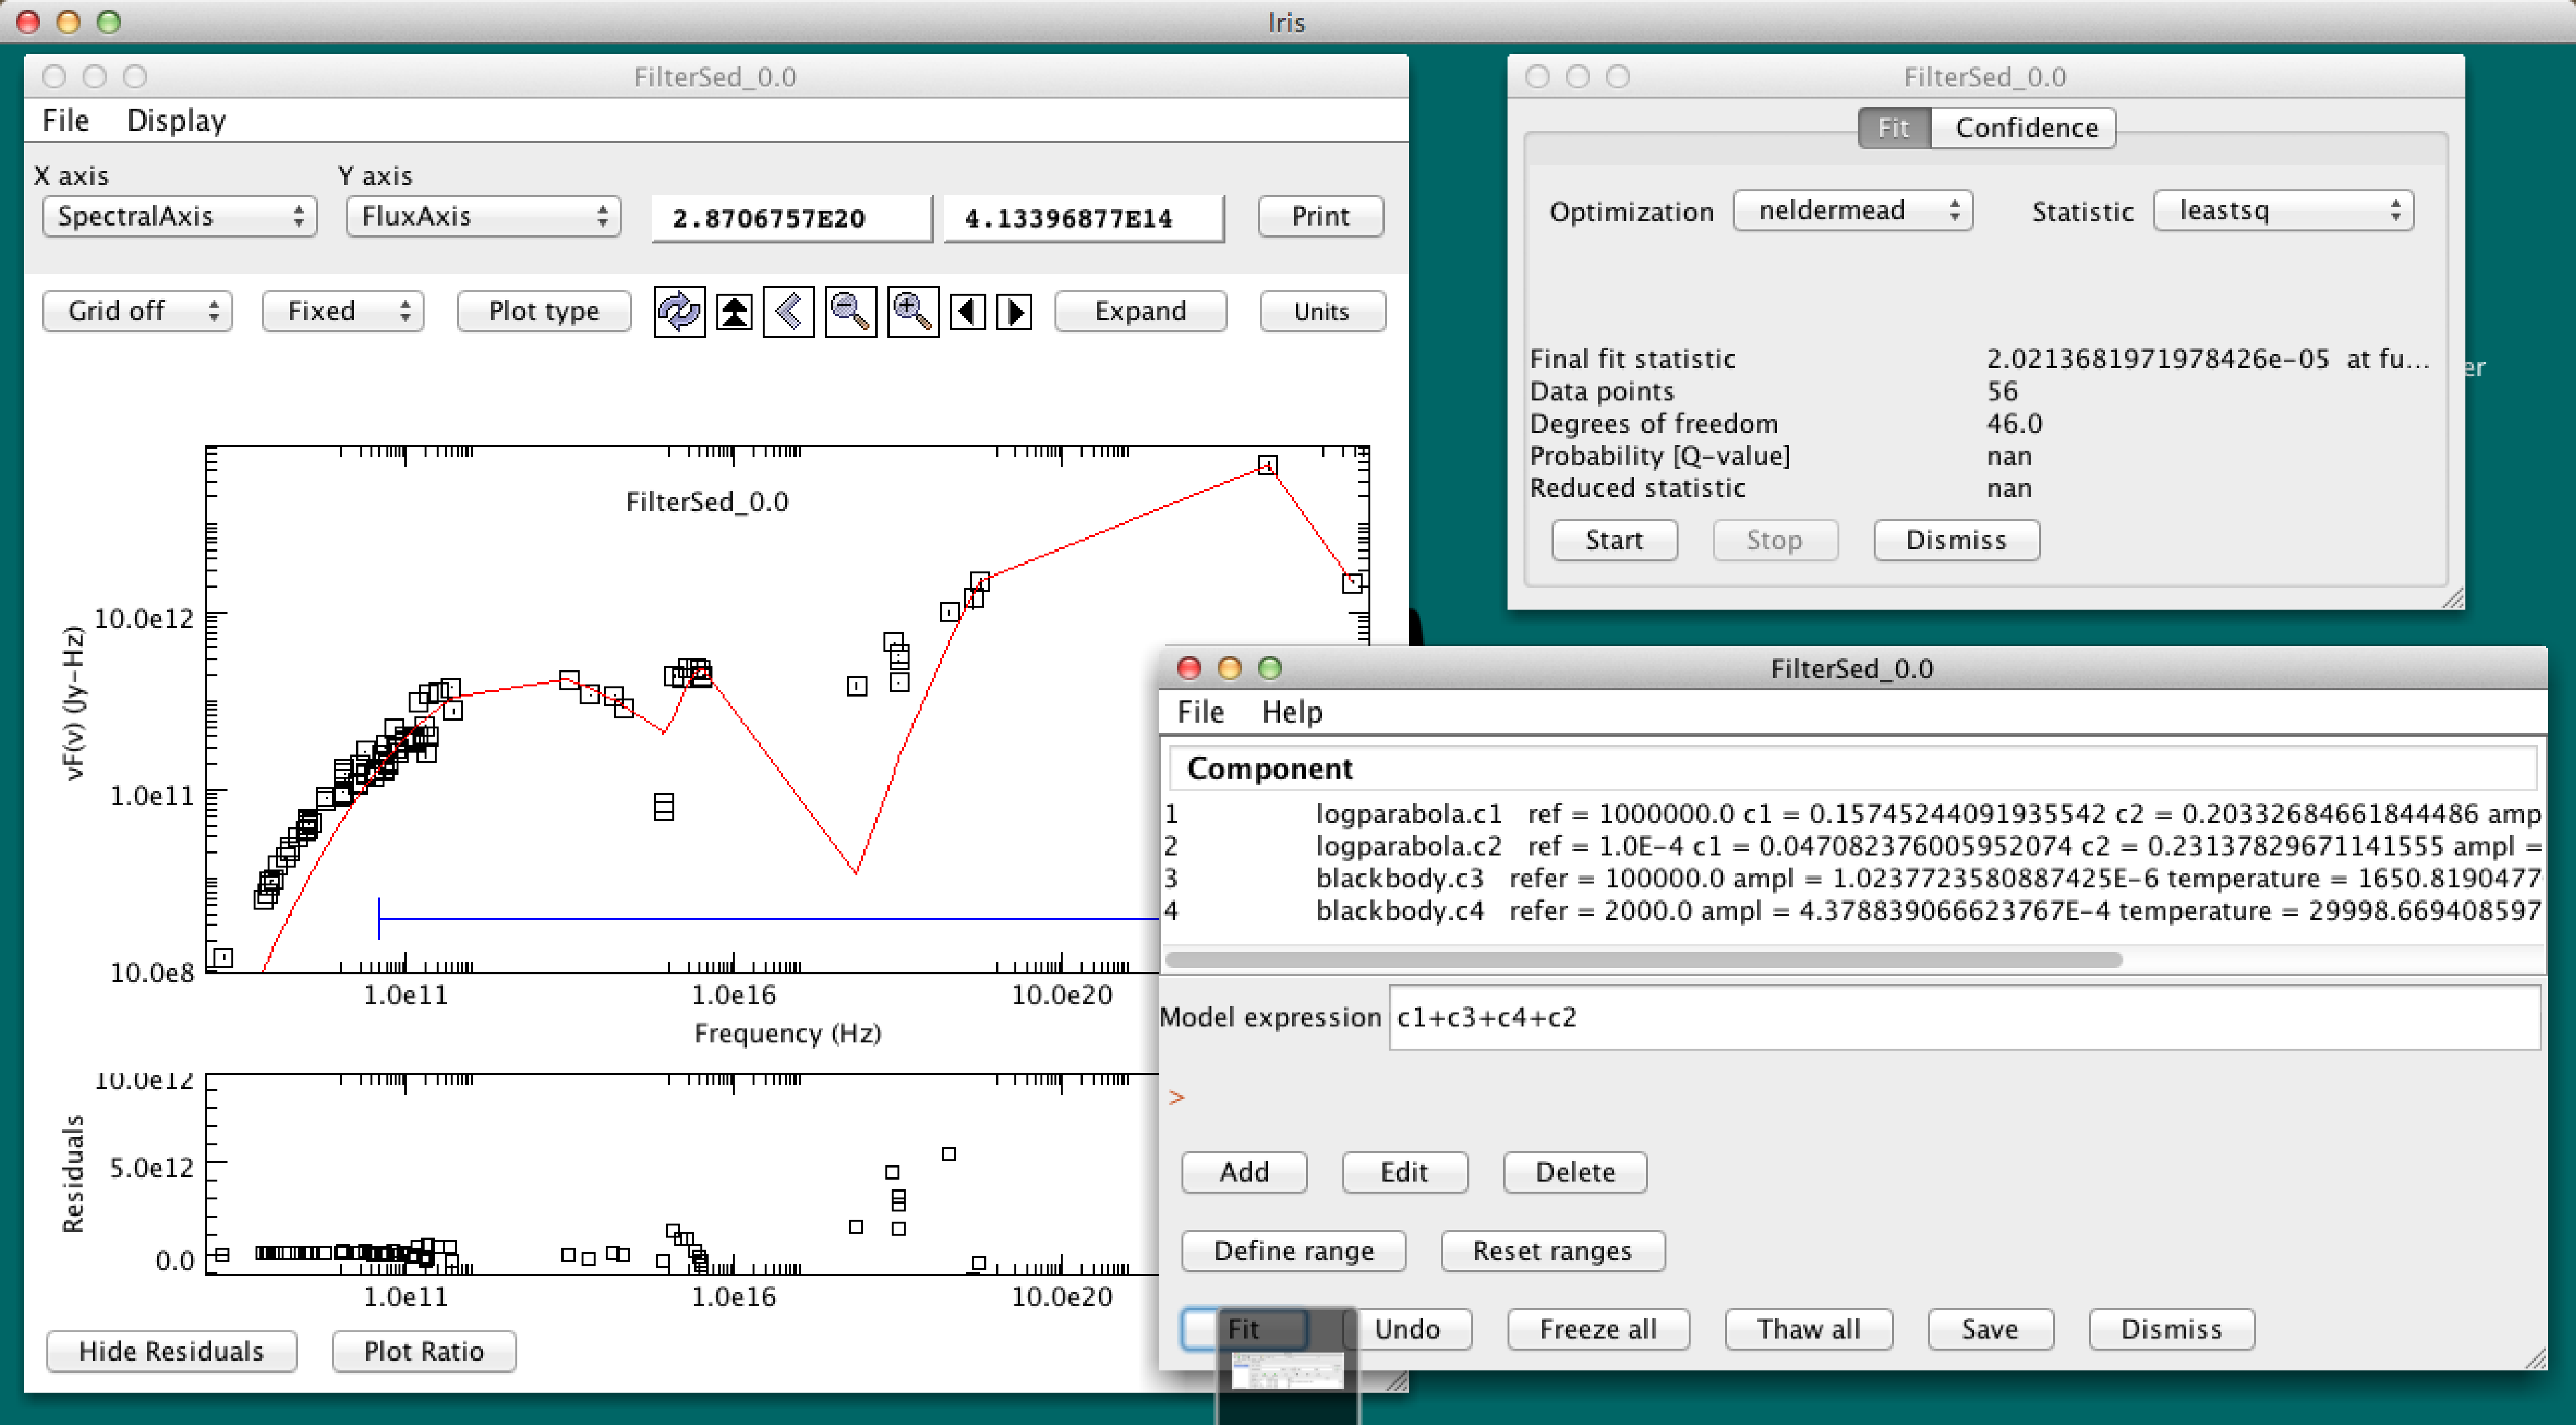
\includegraphics[height=0.3\textheight]{figures/fitting-1.png}
\caption{\textbf{Fitting Visualization} Visualization of a linear combination of log-parabolas and blackbody distributions for FRSQ blazar PKS 1127-145, fit with Neldermead optimization and least-square statistics. \textit{Left:} The best fit linear combination overlaid on the SED data as a red curve. The blue line shows the spectral range over which the data was fit. Below the main plot are residuals of the fitted curve, in dex units. \textit{Top-right:} The fitting options and results. Here, the user chooses between Neldermead, Levenberg-Markwardt, and Monte-Carlo optimization and various least square and $\mathrm{\chi}^{2}$ statisitcs. The fit statistics are reported here after the fit has been performed. \textit{Bottom-right:} The Fitting Tool window. The model components used in the fit and their fitted parameter values are listed in the Components field. Below that is the Model Expression, in which the components are linearly combined. Note that components are referenced by the \textit{c\#} suffix of the component name.}
\label{fig:fitting1}
\end{figure*}

An Iris session begins with populating a SED. A user loads a local ASCII file of PLANCK data, a WISE dataset from TOPCAT~\citep{2005ASPC..347...29T} through a SAMP message, and all data associated with PKS 1127-14 in NED with the NED SED Service portal. She also uses the built-in Italian Space Agency Science Data Center\footnote{http://www.asdc.asi.it/} (ASDC) query tool to find optical/UV data for PKS 1127-14, and adds it to the SED (see Figure~\ref{fig:load_data}).

Data is converted to a single set of units on the fly, and displayed in the SED Viewer. The user can switch the spectral and flux axes between a variety of commonly-used SED units, e.g. one can switch from $\mathrm{Jy}$ vs. ${\mu}\mathrm{m}$ to $\mathrm{Jy}\mathrm{Hz}$ vs. $\mathrm{Hz}$. The Metadata Browser -- an interactive table of the SED data -- allows the user to interactively inspect and filter out data points by hand or with Boolean expressions.

The user also employs the Science Tools, an Iris built-in component that provides operations to redshift, interpolate, and calculate integrated fluxes through photometric filters or user-defined passbands. In particular, the user shifts PKS 1127-14 from its observed redshift at $z=1.18$ to restframe using the Redhisft tool before fitting the SED.

She also filters out all the points devoid of errors using the metadata browser filtering features.

When the user is done building and editing the SED, she begins the fitting session. In the fitting tool, the user can build a model expression as an arbitrary combination of model components. Choosing from a list of astrophysical and mathematical models built-in in Iris, she fits PKS 1127-14 with a linear combination of four models: two logarithmic parabolas to model the radio synchrotron and inverse Compton radiation, and two blackbodies to approximate the models for the hot dust component and accretion disk of the blazar. The fit is performed using Neldermead optimization and least square statistics. The user has fine control over the parameters, including setting initial values, the range of the values, freezing and thawing parameters, and linking model parameters to other parameters in the model expression. The spectral range to which each model component must be applied is also used to make control the fit: finally, confidence interval are computed for the overall model parameters.

Figure~\ref{fig:fitting1} shows the final model for PKS 1127-14 overlaid on the input data and, in the lower panel, the fit residuals.

When the user is satisfied with her fitting results, she saves an XML-style file of the model that can be re-read into Iris and fit to other SED data. She also saves the fit results to a text file, which shows the parameters of the fit and the details about each model component, with the best-fit parameter values.


%\section{Iris Use Case: Fitting a SED}
%\label{subsec:builtin}

%To showcase its main functionalities, we through an example use-case of Iris. We analyze the SED of the flat radio spectrum quasar (FRSQ) blazar PKS 1127-14, and save the results to file.


%\subsection{Building the SED}

%As stated in Section \ref{sec:overview}, Iris can read data from a variety of sources in different formats. Figure \ref{fig:load_data} shows an example session of loading data into Iris. The user loads a local ASCII file of PLANCK data with a built-in file reader. In a TOPCAT~\citep{2005ASPC..347...29T} session, the user completes a cone search of WISE photometry for PKS 1127-14, then broadcasts the data to Iris through SAMP. 

%The user queries NED for photometric data through the NED SED Service portal to see published data for PKS 1127-14. The user sees that she has no optical/UV data in the SED by inspecting her data in the SED Viewer, the interactive data display. She uses the built-in Italian Space Agency Science Data Center\footnote{http://www.asdc.asi.it/} (ASDC) query tool to find optical/UV data for PKS 1127-14, and adds it to the SED (see Figure~\ref{fig:load_data}). 



%%The VO-compliant data is automatically added to the SED Builder and the SED Viewer, the interactive plotting display.

%%The user loads PLANCK data from a local ASCII file, and broadcasts WISE data from a TOPCAT~\citep{2005ASPC..347...29T} cone search via SAMP. As both datasets are non VO-compliant, Iris opens file reader GUIs in which the user provides the mapping for the spectral, flux and flux uncertainties. %The file importers provide helpful hints for the user when filling in the forms.

%%Wanting to see other published data on PKS 1127-14, the user queries the NED database for photometric data through the NED SED Service portal. The VO-compliant data is automatically added to the SED Builder and Viewer, the interactive plotting display. The user then opens the ASDC\footnote{http://www.asdc.asi.it/} query tool to grab data taken with SWIFT and GALEX (see Figure~\ref{fig:load_data}), and imports the data directly to the SED.

%\subsection{Inspecting the SED}
%\label{subsec:inspect-sed}

%She switches the spectral and flux units from $\mathrm{Jy}$ vs. ${\mu}\mathrm{m}$ to $\mathrm{Jy}\mathrm{Hz}$ vs. $\mathrm{Hz}$ (Iris takes care of all unit conversions once the data is read in). The user then shifts the SED from its observed redshift of $z=1.18$ to restframe. Before starting a fitting session, she wants to remove from the SED data without flux-uncertainty measurements. For this, the user opens the Metadata Browser -- an interactive table of the SED data -- and uses a Boolean filter to dynamically select points that have uncertainty measurements. From these selected points, the user creates a new SED object that is managed separately from the original SED. The user saves the filtered, restframe SED to a VO-compliant FITS file, which can be re-read with Iris and other FITS-compliant tools.
% SEDs are saved in VO-compliant FITS or VOTable formats which can be re-read into Iris or other programs (e.g. TOPCAT; IDL or Python interpreters).

%\subsection{Fitting the SED}

%%Blazar SEDs are dominated by two peaks. It has been shown that the low-energy peak, due to radio synchrotron radiation, and the higher-energy bump, due to inverse Compton radiation, can be modeled by log-parabolic distributions \citep{2006A&A...448..861M,2009A&A...501..879T}. Also present in blazars are an accretion disk and a hot dusty torus surrounding the super-massive black hole, both of which can be modeled by blackbody distributions \citep{2002ApJ...575..667D}. The user wants to model the SED pf PKS 1127-14 with a linear combination of these four models.

%The user wants to model the PKS 1127-14 SED with a linear combination of four models: two logarithmic parabolas to model the radio synchrotron andinverse Compton radiation, and two black bodies to approximate the models for the hot dust component and accretion disk of the blazar; both models are built-in with Iris. 

%The user starts a fitting session by opening the Fitting Tool component on the Iris desktop. The SED Viewer appends a graph for the model residuals below the original SED plot. The user adds the four models to the Components field, where she can edit the parameters by setting their inital values, freezing and thawing values, declaring the value ranges, and linking the values to other parameters in the model. 

%Users can combine model functions with other functions and arithmetic terms in the Model Expression field. In this case, the user adds the models one-by-one, defining the data ranges to fit for each component, fitting them, then freezing the component afterwards. For each fit, she uses Neldermead optimization and least squares as the statistic. She then tweaks the paramters some more, fine-tuning her model, and refits the SED until she is pleased with her results (Figure \ref{fig:fitting1}).

%%The user starts a fitting session by opening the Fitting Tool component on the Iris desktop. The SED Viewer appends a plot for the model residuals below the original SED plot. The user adds four built-in models: two logarithmic parabolas (\texttt{logparabola}s) for the radio synchrotron and inverse Compton radiation and two blackbodies (\texttt{blackbody}s) for the hot dust and accretion disk. The models are added to the Components field, where the model parameter values are displayed. The user double-clicks each component to edit their initial parameter values, freeze and thaw them, and set their ranges.
%The user removes the powerlaw component, and adds four models from the Preset Components list: two logarithmic parabolas (\texttt{logparabola}s) for the radio synchrotron and inverse Compton radiation and two blackbodies (\texttt{blackbody}s) for the hot dust and accretion disk. The models are added to the Components field, where the model parameter values are displayed. Double-clicking a component allows you to edit the parameters, e.g. freeze and thaw parameters, reset their initial values, and set their minimum and maximum values.

%%In the Model Expression field, the user linearly combines the models, adding and fitting them one-by-one, defining the data ranges for each component, then freezing the component afterwards. For each fit, she uses Neldermead optimization and least squares as the statistic. She then thaws all desired parameters and refits the entire SED with the same statistic and optimization (Figure \ref{fig:fitting1}).
%In the Model Expression field, the components are combined in arbitrary ways. Each component is given an ID which is used to reference the component in the Model Expression field. The user can also set the data ranges to be fit. In this example, we linearly combine the models, adding and fitting them one-by-one, defining the data ranges for each component, then freezing the component afterwards. For each fit, we use Neldermead optimization and least squares as the statistic. We thaw all components and refit the entire SED; the result is shown in Figure \ref{fig:fitting1}.

%When she is done, the user saves an XML-style file of the model that can be re-read into Iris and fit to other SED data. She also saves the fit results to a text file, which show the fit statistics, models used, and the best-fit parameter values. 

\section{User Models and Templates}
\label{sec:usermodels}

Keeping with our requirements of developing an extensible SED analysis tool, we provide a user-end interface for adding custom models, templates, and template libraries for the fitting engine to use in a Custom Fit Models Manager.

Sherpa, Iris' fitting engine, provides command line functions for users to add their own models and templates to a Sherpa session. We wrap a GUI around such functions for streamlined integration and user-friendliness.
%We wrap a GUI around Sherpa's \texttt{sherpa.astro.ui.utils} functions \texttt{load\_user\_model}, \texttt{load\_table\_model}, \texttt{load\_template\_model}, and \texttt{add\_user\_pars} for streamlined integration and user-friendliness.
The user provides the full path to the directory where the models and templates exist, as well as information about the parameters. Installing a model saves a copy of the model files in the user's home directory (in \~{}/.vao/iris/components), allowing the user to apply the models in future sessions.

%; in this way, both users familiar or unacquainted with Sherpa will

\subsection{Custom Python Functions}
Iris accepts custom models as Python functions stored on the user's disk. Any number of functions can be stored in a single file. The function implementing the model must take two parameters: the first is an iterable of the model parameters, the second is a placeholder for the spectral axis, $x$, in units of Angstroms. For example, a model file for a modified black body
\(B_{\nu}(T) \left(\nu/\nu_{0}\right)^{\beta}\)
could be defined as in Listing \ref{lst:user_model_example}.

User models can be arbitrarily combined with other custom or preset model functions when using the Iris fitting tool.

\begin{lstlisting}[style=python,
	caption={Example of a user-defined model that can be dynamically loaded into Iris. The code implements a modified blackbody and can be combined in Iris with other built-in and custom components.},
	label=lst:user_model_example]
import numpy as np

def modified_blackbody(p, x):
    """
    Modified blackbody of the form:
    A * B_lambda(T) * (c / (lambda / lambda_0))**beta

    Parameters
    ----------
    p : [lambda_0, A, temp, beta]

        p[0] 'lambda_0' : refernce wavelength
        p[1] 'A' : amplitude of model at reference wavelength
        p[2] 'temp' : temperature of blackbody
        p[3] 'beta' : dust emissivity index

    x : array
        spectral values, in Angstroms
    """

    # blackbody function, in terms of wavelength (in Angstroms)
    c1 = 1.438786e8  # in AA K
    efactor = c1 / p[2]
    numerator = p[1] * np.power(p[0], 5.0) * (np.exp(efactor / p[0]) - 1.0)
    denominator = np.power(x, 5.0) * (np.exp(efactor / x) - 1.0)
    B_lambda = numerator / denominator

    # speed of light in Angstroms/second
    c = 2.998e18

    powerlaw = (c / (x/p[0]))**p[3]

    return B_lambda * powerlaw
\end{lstlisting}


\subsection{Table Models}
A table model is a single template, having just the $x$ and $y$ coordiantes. Iris accepts two-columned ASCII files as table models, following the convention where the first column is the spectral values (in Angstroms) and the second contains the fluxes (in $\mathrm{photons}/\mathrm{s}/\mathrm{cm}^{2}/{\AA}$). The fit returns the normalization constant (or amplitude) of the model.

\subsection{Template Libraries}
The template model is essentially a list of table models with parameters other than the amplitude. Like the \texttt{load\_template\_model} function in Sherpa, the user must create an index file which lists the parameter values of the templates and the full path to the template those parameter values describe (see Listing \ref{lst:templateconfig} for an example). Sherpa uses a grid-search method to find the best-fit template.


\begin{lstlisting}[style=code,
	caption=Example of template library definition file,
	label=lst:templateconfig]
# INDEX REFER MODELFLAG FILENAME
0.0     5000  1   /data/sed_temp_index-0.00.dat
-0.10   5000  1   /data/sed_temp_index-0.10.dat
-0.25   5000  1   /data/sed_temp_index-0.25.dat
-0.35   5000  1   /data/sed_temp_index-0.35.dat
-0.50   5000  1   /data/sed_temp_index-0.50.dat
\end{lstlisting}


\section{The Iris Stack}
\label{sec:stack}

The Iris stack (Figure \ref{fig:stack}) shows how one can put the cold and technical IVOA specifications to work for scientists through higher and higher layers of abstraction: the technical details of the Virtual Observatory standards and protocols lie in the bottommost layers, the internals of the Iris building blocks lie in the middle layers, while the topmost layers express high-level user-oriented functionalities.

A reader without any knowledge of programming, let alone of the VO specifications, should understand the labels used in the topmost layers of the diagram and their components (e.g. the Fitting Tool, Redshift), as long as they have some knowledge of astronomical SEDs. On the other hand, a developer would find words like framework, service, and manager quite familiar, while it takes a VO-savvy person to decode the acronyms at the bottom of the diagram.

\begin{figure}
\begin{center}
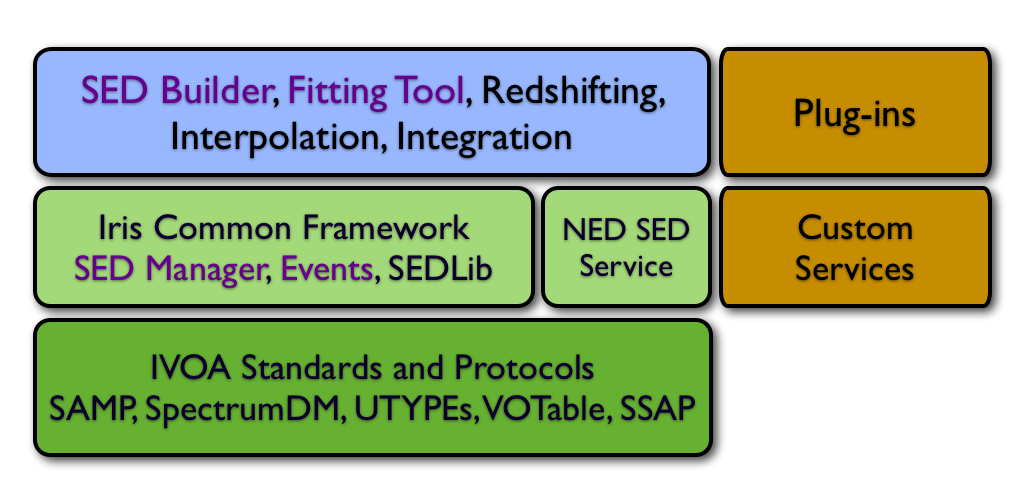
\includegraphics[width=\columnwidth]{figures/IrisStack.png}
\caption{\textbf{The Iris Stack} With its architecture Iris allows developers to create components using higher and highet abstractions on top of web services, desktop applications, and Virtual Observatory standards and protocols. The technical specifications lie on the bottom, a middle layer provides abstractions useful to developers, and the user is only exposed to the science features. Users can also plug their code in as Python functions. The result is aimed to be both user- and developer- friendly.}
\label{fig:stack}
\end{center}
\end{figure}

This fact reflects the different entry points for the different audiences of the application: core developers work at all levels of the stack, but need to lay out the foundations on top of the standard specifications; third party developers use the middle-level abstractions offered by the Iris framework, while end users can limit their interaction to familiar astronomical concepts through the application's user interface. End users can also plug in their modeling code and upload templates libraries to Iris.

The color code in Figure \ref{fig:stack} adds a different dimension to this diagram and taps into a different characteristic of the Iris architecture: extensibility. In particular, blue boxes with purple letters denote extensible components of the architecture, i.e. component that offer hooks into the Iris architecture to users and developers. The orange labels, on the other hand, express components that were not even part of the Iris design, but that can be loaded in Iris as plug-ins, possibly providing an interface to access non-standard services. Some of these plug-ins, along with a description of the design of the Iris Software Development Kit, will be introduced in section \ref{sec:plugins}.

The Iris development team also faced some extra challenges: our team was distributed in nature, with developers and managers working from different institutions with different tools and practices \citep{2012SPIE.8449E..0IE}. Moreover, willing to reuse existing software instead of reinventing the proverbial wheel, we had to integrate different existing software components in a seamless way.

In summary, the Iris framework was designed to address several different requirements: (i) functional requirements gathered by the Iris team's lead scientists; (ii) functional requirements unknown at development-time; (iii) the distributed nature of the Iris development team; and (iv) the willingness to bring existing tools and services together in a single application.

The Iris stack offers a non-technical view of the Iris architecture and design. While it shows effectively how we tried to abstract end users and developers from the VO specifications and from the specifics of the Iris internals, it does not express the technical solutions that we employed to achieve such extensible architecture and to meet the aforementioned requirements. More detail is provided in some of the following sections.



\section{The Iris Architecture}
\label{sec:architecture}

\begin{figure*}
\begin{center}
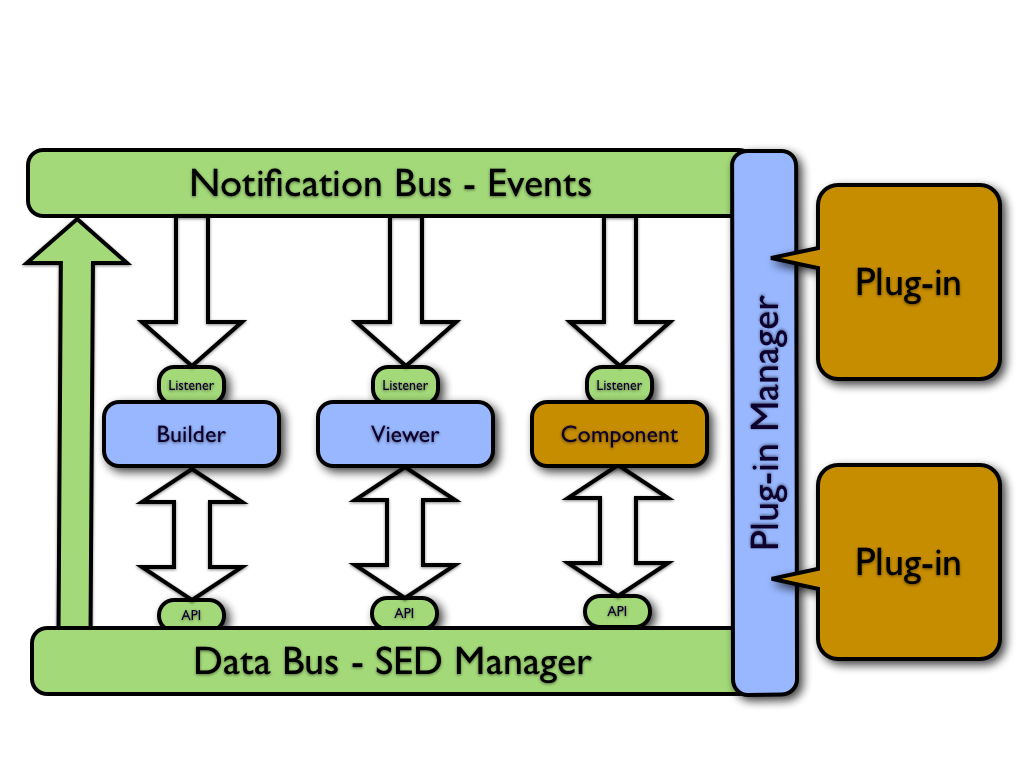
\includegraphics[width=0.6\textwidth]{figures/IrisDiagrams.001.png}
\caption{\textbf{The Iris loosely coupled, extensible architecture} Information freely flows among built-in and third-party components provided as plug-ins. A SED Manager gives components access to the state of the SEDs in the user's workspace, while dynamic changes in such state are announced through events that are notified to the subscribed listeners. A plug-in manager allows users to install and uninstall plug-ins on the fly.}
\label{fig:architecture}
\end{center}
\end{figure*}

\begin{figure*}
\begin{center}
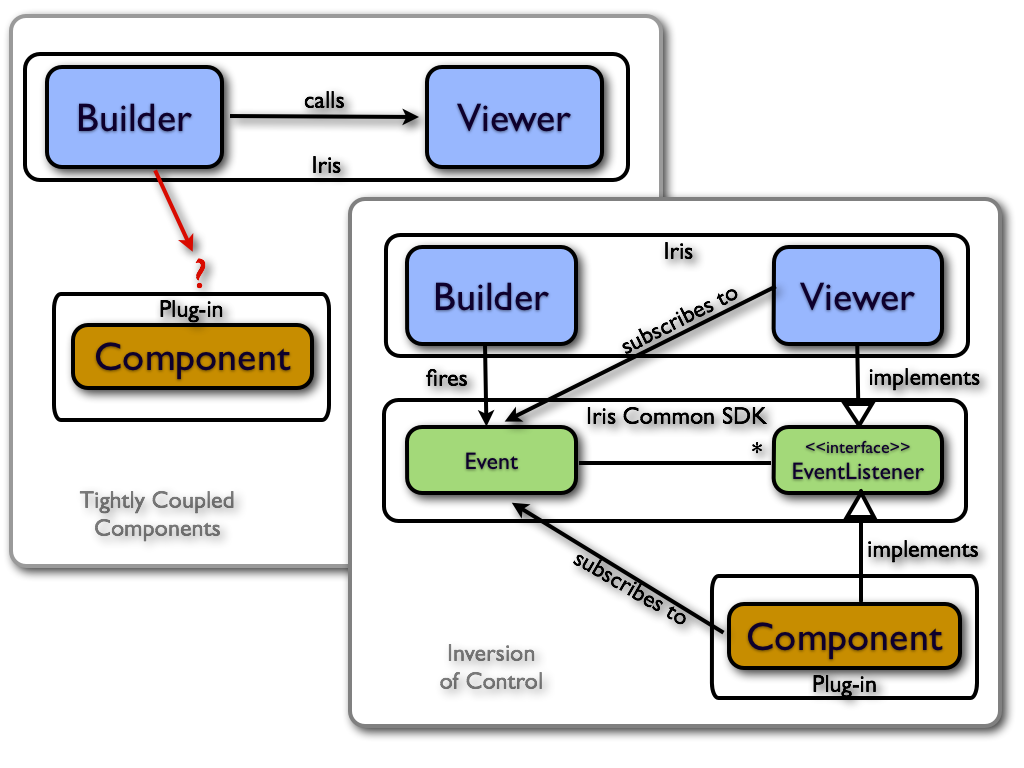
\includegraphics[width=0.6\textwidth]{figures/IrisDiagrams.003.png}
\caption{\textbf{Inversion of Control} IoC is a design pattern that promotes decoupling of software components so that they can easily be replaced by different implementations, with the actual binding often happening at runtime according to some configuration. This pattern, however, also allows new components to be added at any time during the application lifecycle: a common framework (Iris Common) can be shared as a middle layer among implementations, and a container (the Iris application) can bind components together on the fly. Components can subscribe to events and react to them.}
\label{fig:ioc}
\end{center}
\end{figure*}

As mentioned before, Iris was designed to put together existing and newly developed software components in a rich, extensible application. Also, Iris was developed by a distributed team.

In order to minimize the risk deriving from such constraints, we backed Iris with a loosely coupled architecture through a design pattern called Inversion of Control \citep*{ioc}.

But it was not just a matter of risk management: this design pattern also supports the implementation of \emph{liquid} requirements, i.e. a finite set of predetermined requirements plus an undefinite set of custom requirements to be implemented by users, at least in some simple cases or, for more advanced features, by third party developers.

The architecture supporting the implementation of such requirements has different components that can be mapped to the Model-View-Controller (MVC) design pattern:
\begin{description}
\item[SEDLib] a basic I/O library provides classes the Model components of MVC. Unsurprisingly, SEDLib does so by implementing a Data Model specification defined by the IVOA. Such specification defines both the logical breakdown of spectral datasets, and the serialization in some standard file formats. So, on one end, SEDlib can perform the basic read/write operations on spectrophotometric files, while on the other it provides the data structures that client components can use and exchange.
\item[SEDManager] The MVC Controller role is played in Iris by the SEDManager, which is itself defined as an Interface. The manager works as a data storage for SEDLib instances that the different Iris components can share.
\item[Components] The actual Iris functionality is implemented by the Iris Components. They can be seen as the Views in the MVC pattern (or, more generally, they can provide any number of Views), since they present the data stored in the Controller to the user, query the Controller itself, and act upon the Models, i.e. the SED objects provided by SEDLib.
\item[Events] Views can be notified of changes in the Models by Events, if they implement the relative Listener interface and have been registered to the Events Queue. Events usually have a payload with more information about their content, and a pointer to the Model instances involved.
\end{description}

In summary, Components (Views) can be completely disentangled from each other and interact indirectly through the sole common interface represented by the SEDManager (Controller), which in turn stores the SED objects (Model). Dynamic changes in the system are notified to all interested agents (Listeners) via specific Events.

Components are thus agents that cohoperate by attaching themselves to a common \emph{bus} where the SEDManager provides the memory, and Events guarantee the flow of information. (see Figure~\ref{fig:architecture})

\subsection{Inversion of Control}

We achieve loose coupling by an extensive use of Java Interfaces: components, events, and event listeners, for example, are all defined by interfaces whose implementation can, to some extent, be freely interchangeable.

Moreover, Inversion of Control (Figure~\ref{fig:ioc}) is employed to decouple the implementation of components from the run time context: methods in the Interface are callbacks, and some of these callbacks get Interface-typed arguments which provide them context instances during the application execution. For this reason, this pattern is also sometimes referred to as \emph{Dependency Injection}\footnote{There is, to be precise, a subtle but significant difference between Dependency Injection and Inversion of Control, the first effectively being a special case of the second.}.

Consider, for example, Iris Components: they are the main providers of Iris functionality, and they can correspond to buttons and menu items on the Iris desktop, loggers, data handlers, etc. They must implement the IrisComponent interface, which is listed in Listing \ref{lst:component}.


\begin{lstlisting}[style=java,
	caption={This snippet of code represents the main interface that all components in Iris have to implement, and how dependencies get injected into the components at runtime.},
	label=lst:component]
package cfa.vo.iris;

import java.util.List;
import org.astrogrid.samp.client.MessageHandler;

public interface IrisComponent {
    /**
     * This method is invoked to initialize the component. If the component has to launch windows, frames or
     * background services, this is the right method to do so. Otherwise the component will be called only if a callback
     * is invoked.
     *
     * @param app A reference to the running application
     * @param workspace A reference to the application's workspace
     */
    void init(IrisApplication app, IWorkspace workspace);
    /**
     * Return the name of this component. This name might be listed in a widget along with the other registered components.
     * @return The component's name as a String.
     */
    String getName();
    /**
     * Get e description for this component. The description might be listed in a widget along with the other
     * registered components.
     *
     * @return The component's description as a String.
     */
    String getDescription();
    /**
     * Get a command line interface object for this component.
     * @return A CLI object
     */
    ICommandLineInterface getCli();
    /**
     * Initialize the Command Line Application interface
     * @param app Reference to the enclosing application
     */
    void initCli(IrisApplication app);
    /**
     * The component can contribute menu items and desktop buttons to the enclosing GUI applications
     * by providing a list of MenuItems.
     *
     * @return A list of the menu items this component will contribute to the application.
     */
    List<IMenuItem> getMenus();
    /**
     * The component can register any number of SAMP message listeners by providing a list of them.
     *
     * @return A list of the SAMP message listeners that have to be registered to the SAMP hub.
     */
    List<MessageHandler> getSampHandlers();

    /**
     * Callback invoked when the component is shutdown
     */
    void shutdown();
}
\end{lstlisting}

At startup the Iris application reads the list of Components to be initiated, and calls their \verb|init| call-back, which is in turn passed useful information like a reference to the SEDManager, or hooks to the application environment.

The advantages of this architecture are both functional and non functional: it helped our heterogeneous developing team to work in a loosely coupled way, reducing the overall project risk, but it also provides the extensible framework we were seeking in the first place. As a matter of fact, plug-ins that can be loaded at run time implement the same interfaces that the built-in components do, and they are instantiated exactly the same way. The only difference is in the timing: built-in Components get instantiated when the application itself is intialized, while plug-ins can be instantiated and discarded at any time during the application execution.

\section{Iris Built-in Components}
\label{sec:components}
In the previous section, we discussed the architecture of Iris and how the different Components in Iris communicate. Each Component performs one or more SED-related tasks in Iris, like building SEDs from multiple sources and fine-tuned SED modeling.  Here, we discuss what the Components do in terms of the science domain and how they do it, including descriptions of the autonomous software used to build Iris: Specview, Sherpa and the NED SED Service.

\begin{figure*}
\begin{center}
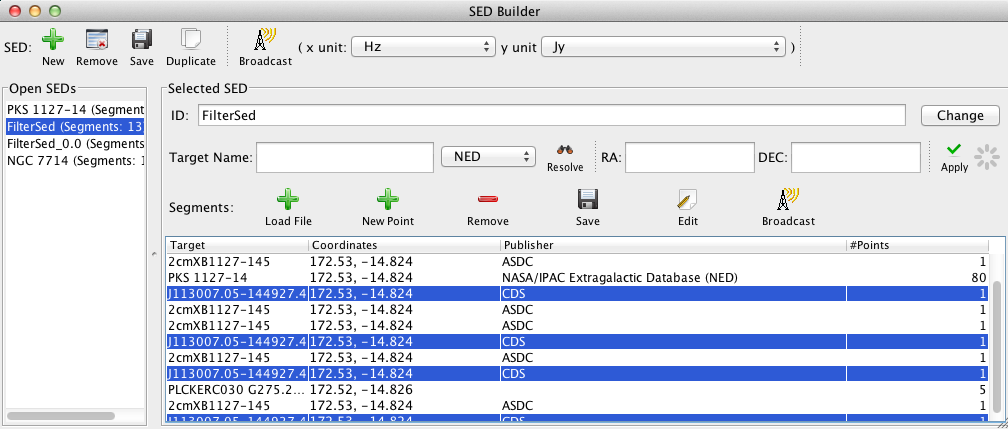
\includegraphics[width=\textwidth]{figures/sed_builder.png}
\caption{\textit{\textbf{SED Builder}} An example view of the SED Builder. On the left side of the window is a list of SEDs open for analysis; in this case, \textit{FilterSed} is selected. The Segments or components that constitute \textit{FilterSed} are shown in the Segments section. Segments may be managed separately. Highlighed SEDs or Segments may be edited, removed, saved or broadcast to an external SAMP-enabled application. New Segments and SEDs are added to the Iris session through the SED Builder. }
\label{fig:sed_builder}
\end{center}
\end{figure*}

\subsection{SED Builder}

Users manage SEDs through the SED Builder (Figure~\ref{fig:sed_builder}). From the Builder, users can add, edit, remove, and save SEDs. Users can also transfer data seamlessly to other VO-enabled applications through SAMP messages from the Builder. Any number of SEDs can be analyzed in an Iris session. Each SED has a unique identifier that is set by default when a new SED is created, but can be changed by the user. The user switches between SEDs by clicking on a SED name in the Open SEDs field; the visualizer will automatically update to the selected SED.

SEDs are built and managed in Segments, which are groups of (spectral, flux) coordinates. For example, a spectrum is considered a Segment; the results of a NED SED Service query are also handled as a Segment. In general, anything from a single photometric point to an entire SED can be considered a Segment, with its points sharing some if not all of the metadata.

Clicking on a SED in the Open SEDs field will show all the Segments that populate that particular SED. SED Builder shows where the Segment data came from, the recorded RA and Dec of the Segment, and the number of points in the Segment. Segments can be handled separately from other Segments in the SED; users can add, edit, remove, and save selected Segments separately from the SED in which it lives.

\subsubsection{Importing data}

\begin{figure}
\begin{center}
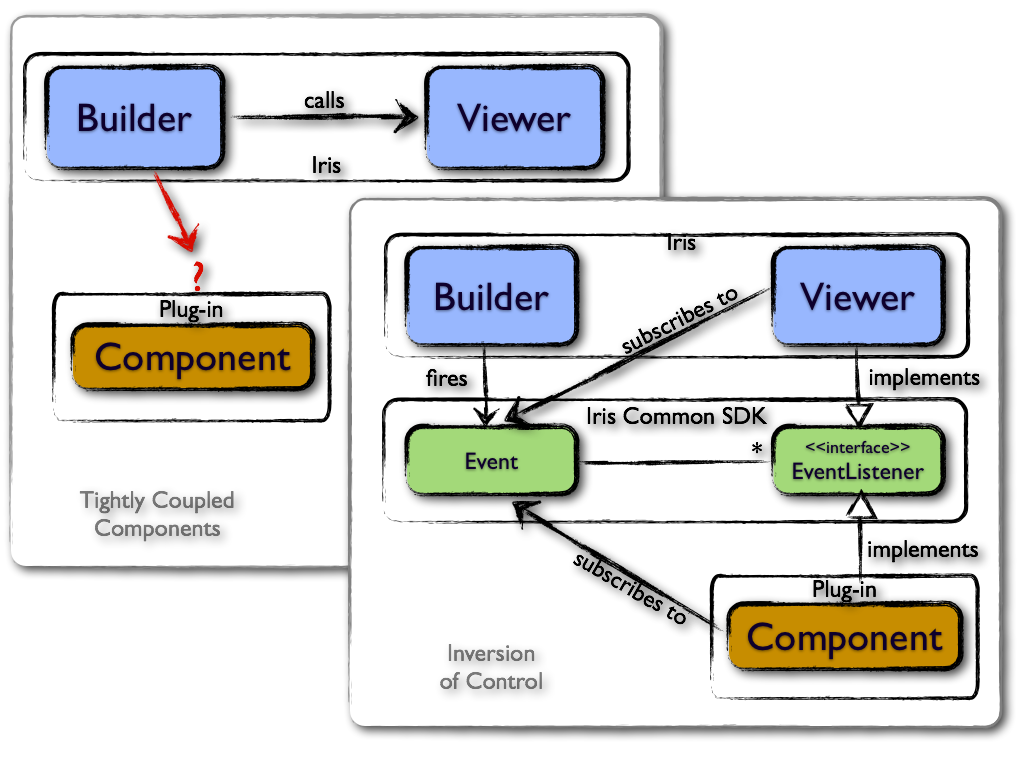
\includegraphics[width=\columnwidth]{figures/IrisDiagrams.002.png}
\caption{\textit{\textbf{\label{fig:data_sources} Available Data Sources}}\textit{}\textbf{}\textit{} Users may import data from the built-in clients to the NED SED Service and the Italian Space Agency Science Data Center (ASDC). Data may also be uploaded from a local file, a URL, a SAMP message from a VO-enabled program (like TOPCAT, CDS Photometry Viewer, or the Data Discovery Tool), or through a custom file filter plugin at run time.}
\end{center}
\end{figure}

As described in Section~\ref{sec:overview}, Iris accepts data from a variety of sources, and is lenient on the data format. Figure~\ref{fig:data_sources} illustrates that Iris imports data from built-in data archive portals as well as from outside resources like local files, URLs, other VO-enabled applications, and from plug-ins.

Iris natively supports IVOA-compliant FITS and VOTable formats (described in \cite{2012arXiv1204.3055M}). Files in these formats will automatically be added to the user's workspace. The Builder can convert ASCII Tables, CSV, Tab-Seprated-Tables, IPAC tables, and non-IVOA-compliant VOTable and FITS files into the native format with user input. We provide two importing forms: (i) the SED importer, which handles spectrum-style files (i.e. those with columns for the spectral coordinate, flux/energy, and flux/energy uncertainties), and (ii) the Photometry Catalog Importer, which handles photometry catalogs (i.e. files where each column represents a passband and the cell values represent the corresponding fluxes, with an arbitrary number of rows). Users can save their setup options from the Import Setup Frame to a configuration file and automatically read-in files of the same format to Iris via the command line.

The SED Builder also has a hook for adding custom file filters. One can develop a custom file reader that would convert a non-standard file to an IVOA-compliant format. This kind of add-on would allow users to automatically read non-standard files into Iris without using the importer tools.

\subsubsection{Saving data}
Users can save entire SEDs or sets of Segments to IVOA-compliant VOTable or FITS files: in order to save all the metadata, the IVOA-compliant serializations rely on some specific constructs in the supported file formats, so that SEDs that have many different Segments can become very complicated to read for VO-unaware applications, although they retain all the metadata details. For instance, segments might have data expressed in different units inside the same SED.

To facilitate the ingestion of SEDs in VO-unaware applications and user scripts, we provide a simpler output format that only saves the minimum amount of meaningful information: the spectral coordinate, the flux or energy, and its uncertainties. The user has to define the units in which all the data will be converted to in the output file. As a result, the resulting SED file has only one Segment.

Whether the output includes all of the metadata or has a simplified \emph{single table} format, the result is a compliant file that can be read back into Iris without any additional user's input.

This allows users to save a standardized version of the file that can be easily shared by Iris and by the user's scripts.

\subsection{NED SED Service}
\label{subsec:ned}

Iris is packaged with a portal to the NED SED Service\footnote{http://ned.ipac.caltech.edu} which, given a target name, retrieves all photometric data in NED associated to the source with that target name, storing it as a SED Segment.

In the context of the VAO development of Iris, the NASA/IPAC Extragalactic Database (NED) adapted its long standing photometry and spectral energy distribution (SED) service to conform as closely as practicable to the relevant IVOA recommendations in order to seamlessly deliver photometric data from the collection into Iris. The objective for NED was to provide a working reference service for the development of Iris as well as to serve as a working prototype for new data protocols for spectro-photometric data being developed by the IVOA.

The NED SED Service returns data and information from the NED photometry collection \citep{2007ASPC..376..153M}. The NED SED Service provides three types of query:
\begin{description}
 \item[Information Discovery] List objects with available photometry (SED) given a sky position (RA and Dec) and angular size.  Also called a \emph{data discovery} query.
 \item[Information Availability] For a given named object (`Target'), how many SED photometric data points are available, if any.
 \item[Data Retrieval] For a given named object, return the available photometric data in an IVOA Spectrum Data Model compatible VOTable.
\end{description}

HTTP requests and responses conform to the IVOA Simple Spectral Access Protocol Version 1.04 (SSAP;~\citep{2012arXiv1203.5725T}), with VOTable responses. Iris employs the Data Retrieval query in its NED SED Service client, and stores the response as a Segment. Photometric points with spectral line-based values and upper- and lower- limit values are excluded from the response.

Since it implements a standard protocol interface, the NED SED service is also available through generic VO applications like TOPCAT and the VAO Data Discovery Tool\footnote{http://vao.stsci.edu/portal/Mashup/Clients/Portal/DataDiscovery.html}.

\subsection{SED Viewer}
\label{subsec:specview}
% insert picture of Viewer with metadata browser open.
The Iris Viewer component is responsible for creating, managing, and providing user interactive feedback to spectral plots in Iris.

The Viewer also provides most of the low-level graphics user interface (GUI) components used by the Fitting Tool component. The reason for this is that most, if not all of the GUI code used by both the Viewer and the Fitting Tool, were developed on top of the Specview~\citep{2002ASPC..281..120B} code base.

Specview was developed in the late 90's, initially as an experiment to evaluate Java graphics capabilities in the context of interactive spectral plotting. Over the years Specview grew from a simple visualizer dedicated mostly to plot spectral data from Hubble Space Telescope (HST) instruments, to a more capable tool with not only sophisticated visualization, but also data analysis capabilities. The ability to ingest spectral data from a variety of sources was also gradually incorporated into the tool, culminating with a Virtual Observatory interface capable of accessing services that comply to the SSAP (Simple Spectrum Access Protocol) standard.

Specview however kept its emphasis on spectral data that is very different from the broad-band SED concept to which Iris is dedicated. Being initially conceived as a tool to support HST data, its design, and subsequent code implementation, were driven by the needs and requirements imposed by high-dispersion, relatively narrow-band spectra in the near-IR / optical / near-UV range. Thus some re-work was necessary to make its internal data structures and algorithms comply with the data types associated with SEDs. Even so, a significant part of the code could be kept as is, thus realizing the savings associated with code re-use. This is particularly true in the case of the low-level graphics engine~\citep{2000ASPC..216...79B}. Most of the work in adapting Specview's code base to Iris happened on two fronts: (i) adding code that implements the Iris Component interface, and (ii) augmenting the capabilities of the Data Browser to allow interactive access to SED metadata. Some work was also done in fine-tuning plotting capabilities to the particular needs of SED data.

The initial view the Viewer creates of a just-ingested SED is via a scatter plot depicting wavelengths (frequency and energy units are also supported) and flux density (or flux) for each data point that comprises the SED. The plot can be configured in a variety of ways, by changing the scaling and units. The data initially plotted can then be further examined in more detail, using tabular and tree depictions. In particular, the metadata associated with each data point, as well as the global metadata associated with the entire SED, can be examined in detail using the Metadata Browser. Data points can be selectively removed from the SED using filters sensitive to both data and metadata values. These filters are built by a user-defined boolean expression that can be created and interacted with in the GUI itself. The expression uses Python-like syntax, and Python operators are available throughout. That way, SEDs can be modified after being read by the SED Builder, and before being further processed or measured.

\subsection{Sherpa: Model Fitting}
\label{subsec:sherpa}
Sherpa is the CIAO modeling and fitting application. It enables the user to construct complex models from simple definitions and fit those models to 1D (spectra) and 2D (images) data, using a variety of statistics and optimization methods.

Written in Python, with C/\Cpp/Fortran extensions, Sherpa was a robust choice for providing Iris with a curve fitting engine.

However, since the Iris front end was going to be a Java application\footnote{In the first version of Iris the front end was a modified version of Specview itself, while in later versions we integrated different components under a common framework graphically represented by the Iris Desktop. Even in this configuration, the fitting front end was provided by Specview under the hood.}, an interoperability layer had to be designed to interface the graphical user interface and Sherpa as a fitting engine backend.

SAMP is used as the interface protocol: this decision makes the design of the interface very simple, so that the interoperability layer on top of Sherpa is rather thin and consists only of the code required to inspect the incoming SAMP messages and build a call to Sherpa.

\begin{figure*}
\begin{center}
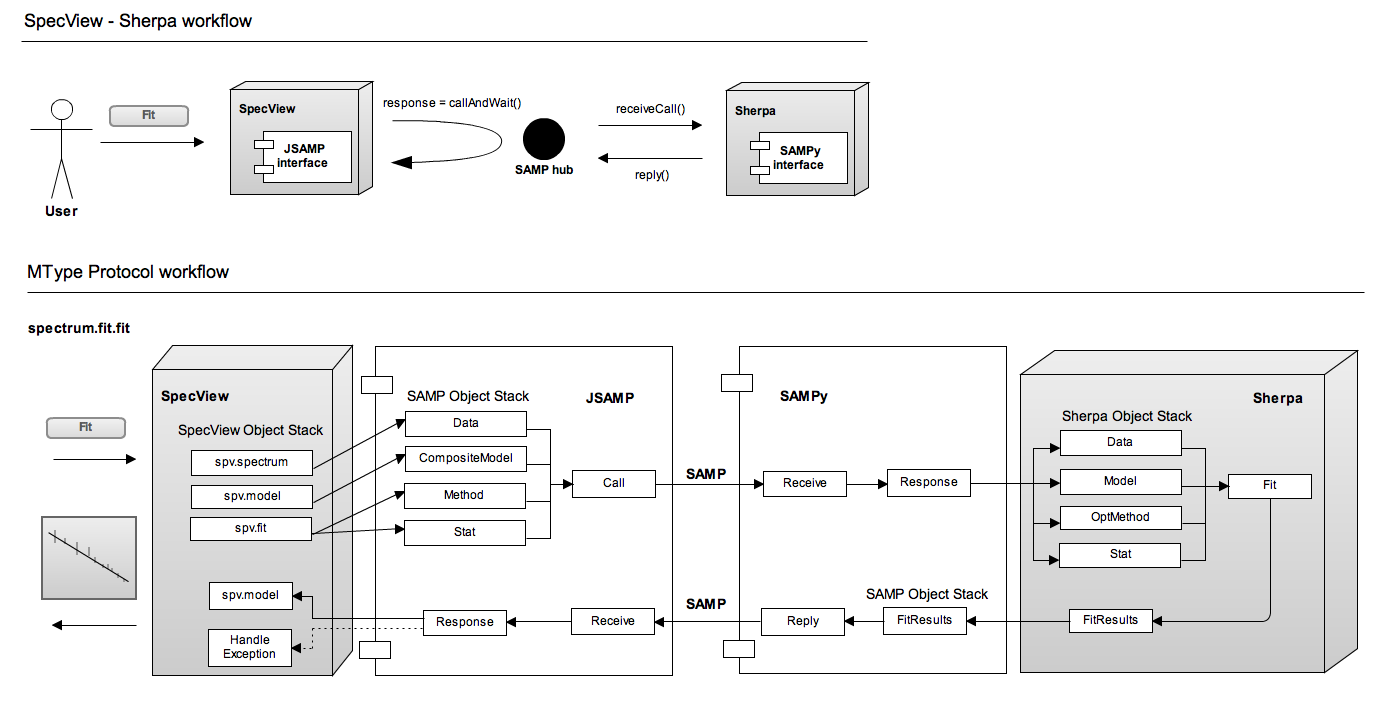
\includegraphics[width=\textwidth]{figures/sherpasamp.png}
\caption{\textbf{Design of the Specview/Sherpa interoperability layer} The interface between Sherpa (fitting engine), and Specview (graphical user interface) was designed by defining a common data model for representing the requests and responses of fitting operations: the serialization of the request is a SAMP message, whose \texttt{mtype} identifies the remote operation that the client is requesting.}
\label{fig:sherpasamp}
\end{center}
\end{figure*}

The design of this interface is represented schematically in figure \ref{fig:sherpasamp}.

When Iris is launched the \verb|sherpa-samp| process is also started in the background: this process implements a SAMP client that waits for a SAMP hub to be available and attaches to it, registering to a number of custom \verb|mtypes|. The \verb|mtypes| work as remote procedures identifiers, and SAMP messages provide the remote methods with data that needs to be processed. Sherpa is used to crunch the data and the response from Sherpa is again packaged into a SAMP message response, so that it can be shown to the user.

The thin layer between Java and Python code is implemented using two existing implementations of the SAMP protocol, namely \verb|jsamp| for Java and \verb|SAMPy| for Python.

The \verb|sherpa-samp| layer grew to accommodate the new science requirements in the latest Iris releases, and it now includes some analysis code that is independent of Sherpa.

\subsection{Science Tools}
We provide built-in science tools that perform calculations commonly used in SED analysis: redshifting, interpolation, and integration. The data is setup on the Java-side of Iris, but the actual calculations are done in \verb|sherpa-samp|.

The open SEDs are listed in the Science Tools frame. The user selects the SED they wish to analyze, and inputs the required information for a calculation.

\subsubsection{Redshifting}
Redshifting an SED in Iris refers to cosmological redshift. Because the apparent magnitude of a source is dimmer at high redshifts than low redshift, we correct the flux so that the area under the shifted SED equals that of the un-shifted SED:

\begin{equation} \label{eq:redshift}
f_{z_{f}}(\lambda) = f_{z_{i}}(\lambda) \frac{\sum_{k=1}^N (f_{z_{i}}(\lambda_{k+1})+f_{z_{i}}(\lambda_{k}))}{\sum_{k=1}^N (f_{z_{f}}(\lambda_{k+1})+f_{z_{f}}(\lambda_{k}))},
\end{equation}

where $f_{z_i}$ is the observed flux at the initial (observed) redshift $z_i$, and $f_{z_f}$ is the flux at the final (target) redshift $z_f$. In \verb|sherpa-samp|, we extend the astLib\footnote{http://astlib.sourceforge.net/} \textit{astSED} class which implements Equation~\ref{eq:redshift}.

From the user's perspective, she supplies the initial and final redshift of the SED and clicks ``Create New SED''.

\subsubsection{Interpolation}
Iris provides 1D interpolation along the spectral axis. There are three interpolation options: linear, linear spline, and nearest neighbor. Interpolation may be carried out on a linear or logarithmic scale. Users may choose the number of bins, the spectral range over which to interpolate, and may choose to smooth the resultant SED via a boxcar method.

\subsubsection{Integration}
The Integration tool was developed to make estimating integrated fluxes of a SED quick and painless. Iris provides two methods of integration: (i) through a user-defined passband, and (ii) through a photometric filter. The first option lets the user specify the spectral range in wavelength, frequency, or energy units (Angstroms, Hz, and keV, respectively) to integrate under. The second estimates the integrated flux measured through any of the photometric filters provided by the Spanish Virtual Observatory's (SVO's) Filter Profile Service\footnote{http://svo2.cab.inta-csic.es/theory/fps/index.php} \citep{2013arXiv1312.3249S}. We chose the SVO's Filter Profile Service because of its extensive collection (over 1000 filters at IR, optical and UV instruments) and of its VO-compliancy. The user chooses from a list of filters which can be searched by double-clicking on an instrument name, or by searching for a string in the browser. The user sees the min, max and effective wavelengths of the filters before applying the filter to the SED.
%How does it work in the background??
Both methods return the effective wavelength of the passband in Angstroms and the calculated flux in Janskys. The user can export the data to a new SED or save the results to a simple ASCII formatted file.

\section{Plug-ins: the Software Development Kit}
\label{sec:plugins}

Iris offers a Software Development Kit (SDK) that can be used to extend the Iris capabilities through the use of dynamically pluggable add-ons, or plug-ins.
The use cases for this are basically two:
\begin{description}
\item[New functionality] A developer may want to create SED-related capabilities in one or more new Components. This use case can be broken down in more detailed and concrete extensions, described later in this section.
\item[Custom-to-Standard adapters] A developer may want to create adapters that query a non-standard service, or load a non-standard data set, and then turn the data to SEDLib objects, thus effectively standardizing them so that they can be used by other components in the Iris environment, or reused by other VO applications. In other terms, one can achieve interoperability using the Iris infrastructure starting from a non-interoperable service, file, or tool. Iris actually has some built-in Custom-to-Standard adapters, like the sherpa-samp layer described in section \ref{sec:components}, or the ASDC plug-in interface that queries a quasi-standard service, described in section \ref{sec:asdc}.
\end{description}

\subsection{Anatomy of a Plug-in}
A single Jar file can archive several plug-ins, and each plug-in can bundle several Iris Components.

Each Component can provide several additions to Iris, as described in some detail below:

\subsubsection{Menus and Buttons}
Usually, although not always, an Iris Component is visible to the user as either a set of buttons on the Iris Desktop, or as a set of menu items in the Iris menu bar, or both.

Menu items can be added to either the File menu or to the Tools menu in a specific plugin-related folder.

While the implementation of such buttons and menu items could be done from scratch by implementing some Java Interfaces, a set of abstract classes implements a lot of the boiler plate code and makes some convenient assumptions. This way buttons and menu items can be created with very few lines of code.

Menu items and buttons can be customized by providing the button name, a description that will be rendered as a mouse-hover tooltip, and icons.

\subsubsection{Command Line}
Iris offers a framework for providing simple command line interfaces to its tools. For example, Iris ships a command line interface to the SED Builder (see Section \ref{sec:components}) that allows users to import non-standard files in bulk through scripts, possibly starting from templates saved interactively from the SED Builder.

This framework is extensible through a simple dispatching mechanism. Each component has a name that is used to dispatch the command line argument to the right CLI engine. For instance, the line \verb|./Iris builder config.txt| instructs Iris to dispatch the \verb|config.txt| argument to the SED Builder's CLI engine.


\begin{lstlisting}[style=java,
	caption={Every Iris component can expose a command line interface. Iris dispatches the command line arguments for the relative component to process.},
	label=lst:cli]
package cfa.vo.iris;

/**
 * A simple interface for providing CLI access in an extensible, pluggable way
 * @author olaurino
 */
public interface ICommandLineInterface {
    /**
     * The name that has to be associated with the implementing component.
     * When the calling application parses the command line, it will interpret the
     * first argument as the component to which the command has to be relayed, using this string
     * as a key.
     *
     * @return The compact name that identifies this CLI
     */
    String getName();
    /**
     * Callback that gets called when a command line is parsed and associated to the implementing component.
     *
     * @param args The command line arguments.
     */
    void call(String[] args);
}
\end{lstlisting}


Components bundled with plug-ins can provide such an engine by implementing the ICommandLineInterface Java Interface (see Listing \ref{lst:cli}).

\subsubsection{SAMP Handlers}
A possible extension that plug-ins can offer to the users is SAMP Handlers: when Iris receives a SAMP message that matches the Handler's \verb|mtype|, the message is directly dispatched to the Handler itself by the Iris framework. As a matter of fact, Iris just offers a convenient shortcut to the excellent \verb|jsamp| implementation of SAMP, making it available to the users with just the bare minimum amount of work required: the setup of the SAMP infrastructure through \verb|jsamp| is all done by Iris, including a keep-alive mechanism that brings a SAMP Hub up if one is shutdown.

A hook is provided for Components willing to send their own SAMP messages to the SAMP Hub, again as a convenient shortcut to \verb|jsamp|.

\subsubsection{Custom Events}
The Iris Events Framework is itself extensible: this way plug-ins can, if needed, create their own nested loosely coupled architecture for their own Components.

\subsubsection{SED attachments}
Components can attach arbitrary objects to the SEDs managed by the SEDManager. This way they do not have to independently manage the additional information they might want to store about the individual SEDs. When SEDs are deleted, the manager takes care of releasing any references to the attachments, so to avoid memory leaks.



\subsection{Plug-in examples}
\subsubsection{ASDC --- stable}
The Italian Space Agency Science Data Center (ASDC) hosts a database with tens of catalogs in a very wide range of wavelengths, also providing time domain information.

A plug-in for providing Iris with a rich graphical user interface to query their database was developed by the ASDC in a collaboration between the ASDC and the Iris teams. The plug-in became part of the main Iris distribution in v2.0 and provided a valuable test bench to review, validate, and improve the Iris Software Development Kit.

While the ASDC data query tool is now part of the Iris distribution, it still provides a very good example of how a plug-in can be integrated seamlessly in the Iris framework to add specific value to it. Integration can be so seamless, actually, that including the plug-in into the main Iris distribution is almost exclusively a matter of configuration rather than of coding.

The ASDC data query tool extends the capabilities of the SED Builder by providing a rich graphical user interface that allows users to check what archives to query, and since the ASDC query is a positional cone search, the client provides different adjustable search radii for each catalog which default to reasonable values consistent with the resolutive power of the individual instruments.

Moreover, the tool allows to query for specific observation time ranges, thus allowing basic time domain analysis of the SEDs.

This component proves several points about the Iris framework and SDK:
\begin{description}
\item[Custom-to-Standard adapters] The ASDC web service backing up the implementation of the query tool does not comply with any VO data access protocols (at least not yet), as it was designed as a private interface to their database to be consumed by a dedicated client. The client on the Iris desktop assumes that the service implements the private interface, and can query it. The data files coming from the service, on the other hand, are compliant with the IVOA specifications, so they can be directly read by SEDLib and passed to the SEDManager.
\item[Interoperability] Although the ASDC plugin was not designed as part of Iris, it integrates seamlessly with the Iris built-in components. When the ASDC query tool instantiates an SED from the service, this gets listed in the SED Builder and visualized in the SED Viewer, even though it does not interact directly with any of them: they all interact only with the SED Manager and they get notified of changes by the events that are fired when Models are changed.
\item[The Iris SDK] As it will be explored in some detail in section \ref{sec:writeplugin}, a plug-in developer can pretty much focus on the implementation of her components' business logic, without worrying too much about the boiler plate code required to configure such components. By using the abstract classes that the Iris framework
provides, one can leverage the existing components with just a few lines of code and then start adding value to the entire application.
\end{description}

\subsubsection{Vizier --- experimental}
\label{sec:asdc}
Experimental plug-ins are shipped with Iris but they can only be activated by turning on switches on the Iris command line. For instance, if one starts Iris with the command \verb|./Iris --vizier| an experimental plugin for the CDS Vizier photometric service gets loaded in the usual Iris desktop.

While this component is, at the time of this writing, still experimental, it shows some properties of the Iris framework and SDK.

As for the ASDC plug-in, this component shows that one can use Iris and its framework to rapidly build an adapter from a dedicated service interface, leveraging the particular specs of the service, so to make datasets interoperable with the other Iris tools, third party plug-ins, and possibly other VO tools.

\subsubsection{R --- experimental}
A highly experimental proof-of-concept plug-in was developed to explore the possibility of interfacing Iris with rich analysis environments like R. The plug-in shows how one can \emph{beam} data from Iris to R and trigger some analysis on the dataset in R.


\subsection{Other Extensibility Points}

\subsubsection{Custom File Readers}
Iris supports a fair number of {fi}le formats natively: VOTable,
FITS, CSV, TSV, ASCII, and IPAC tables. However, new {fi}le {fi}lters can be created and
loaded at runtime. One can also create {fi}lters for the natively supported {fi}les: in this
case, the custom {fi}lter would parse the {fi}le and map the metadata to the IVOA Data
Model {fi}elds.

\subsubsection{Persistence}
Components can also get a handle to the configuration directory, usually a hidden folder in the user's home directory, if they need to persist information like user's preferences, local databases, or work sessions.



\subsection{How to write an Iris plugin}
\label{sec:writeplugin}
Iris uses Maven Archetypes to streamline the process of building and distributing Iris plug-ins.

You might also write plug-ins without using Maven, but you would need to take care of many steps that the Maven-generated project automatically takes care of, like the inclusion of your dependencies in your plug-in's jar file.

In order to have a test plugin up and running you need to create a new project from the Maven archetype:

\begin{lstlisting}[style=code]
$ export repo=http://vaotest2.tuc.noao.edu:8080/artifactory/

$ mvn archetype:generate\
   -DarchetypeRepository=$repo\
   -DarchetypeArtifactId=iris-plugin-archetype \
   -DarchetypeGroupId=cfa.vo \
   -DarchetypeVersion=1.1
\end{lstlisting}

The above command will ask you some questions about the metadata for your plug-in project, like the group id, the project id (called artifact-id in Maven), and the version. At the end of the process you should have a directory named after your project-id. This directory contains all the files needed to build and package a test plugin.

You can type \verb|mvn package| from the newly created directory and Maven will package the test plug-in for you in the \verb|target| directory as a jar file.

You can use the Iris Plugin Manager component to install this jar file into Iris. As soon as you do it, a new button should appear on the Iris desktop. If you click on it, a rather impressive dialog box with the universal salutation ``Hello World!'' should appear on your screen.

You can inspect the source code of this project and notice that most of it is made of metadata strings and basic class definitions and instantiations. By inheriting from the abstract classes that are provided with the Iris SDK, the actual code that one needs to implement starts from the implementation of the \verb|onClick| callback of the AbstractPluginMenuItem class. From that call on, a plug-in developer can focus on the implementation of their components and start using the hooks provided by the Iris Framework in order to interoperate with the other Iris components, and possibly with other VO applications.

One can start from this dummy project, inspect the source code, make changes to the package and class names and to the metadata strings, and then start implementing their component's business logic and user interface.

The Iris website contains further documentation on how to write plug-ins, and you can contact the authors of this paper for further information.

\section{Future Plans}
We are working on improving Iris in several ways. With the VAO shutting down in 2014, the development of Iris has been taken over by the Chandra CXC group at SAO.

While the current Software Development Kit is very advanced for letting plug-ins contribute SEDs and SED segments to the user's workspace, we want to improve the ways in which plug-ins can interact with the visualization and fitting code, decoupling Specview and Sherpa.

We are also exploring solutions to overcome one of the limitations in the current code, namely the handling of high resolution spectra, that is mostly due to a visualization issue.

Several improvements will derive from the inclusion in Iris of the latest Sherpa version, and in particular of the new code for interpolating templates in template fitting. This will allow users to combine templates with other templates and functions and compute photometric redshifts through template fitting, for instance.

Also, we want to provide finer grained control over the visualization and manipulation of individual components in the model expressions.

From the user interface point of view, we are planning to provide Python bindings to enhance the integration of Iris in customized, complex scientific workflows.

\section{Conclusions}
\label{sec:conclusions}

Iris is a Virtual Observatory application designed with the goal of streamlining the construction of broadband spectral energy distributions while providing flexible and robust tools for their analysis, with a stress on interoperability and extensibility.

To summarize, Iris provides: built-in capabilities for building, viewing, and analyzing broad-band spectro-photometric SEDs; a Python framework for fitting user-provided models and templates; interoperability with Virtual Observatory tools through the Simple Messaging Application Protocol (SAMP).

The Iris layered architecture takes advantage of the Virtual Observatory standards and protocols without exposing their complexity to the final users, who still benefit from the added interoperability. At the same time, developers can use a middle layer of abstraction that exposes the domain objects, i.e. spectro-photometric SEDs, and the user's workspace, in a clean and consistent way through a Java software development kit.

This way Iris combines several existing software components with new dedicated software, and provides hooks for astronomer and software developers that want to leverage the general interoperable framework while pluggin in their own code.

Iris is available as an Open Source project, and can be downloaded as a binary or source distribution for Linux and Mac OS X.


\section*{Acknowledgements}
Support for the development of Iris was provided
by the Virtual Astronomical Observatory contract AST0834235. Support for Sherpa is
provided by the National Aeronautics and Space Administration through the Chandra
X-ray Center, which is operated by the Smithsonian Astrophysical Observatory for
and on behalf of the National Aeronautics and Space Administration contract NAS8-
03060. Support for Specview is provided by the Space Telescope Science Institute,
operated by the Association of Universities for Research in Astronomy, Inc., under
National Aeronautics and Space Administration contract NAS5-26555. This research
has made use of the NASA/IPAC Extragalactic Database (NED) which is operated by
the Jet Propulsion Laboratory, California Institute of Technology, under contract with
the National Aeronautics and Space Administration.

\bibliography{aciris.bib}

\end{document}

